%! Author = amatarazzo
%! Date = 06/04/24

\chapter{Foundations of Large Language Models}
\label{ch:foundations-of-large-language-models}

\section{Introduction}
\label{sec:ch2-introduction}

Large Language Models (LLMs) have revolutionized the field of Natural Language Processing (NLP) by achieving state-of-the-art performance on a wide range of tasks, such as text generation, text classification, and machine translation.
These models are trained on vast amounts of text data to learn the underlying structure of the language and capture the relationships between words.

In the following sections, we will explore the key concepts and techniques that underpin the development of LLMs, including pre-training strategies and major datasets used for training and evaluation, as well as the Transformer architecture, which forms the basis of many modern LLMs.

After that, we will discuss some model adaptation techniques that can be used to fine-tune LLMs for specific tasks or domains.

Finally, we will discuss tuning and quantization of LLMs, techniques used to reduce the model's size and computational complexity, making it more efficient for deployment on resource-constrained devices.

\section{Pre-training}
\label{sec:pre-training}

Pre-training constitutes a foundational phase in the development of Large Language Models (LLMs).
It allows the model to capture the relationships between words and generate coherent and contextually relevant text, laying the groundwork for its subsequent performance on specific NLP tasks~\cite{devlin2019bert, brown2020language}.
This phase involves training a language model on a vast corpus of text data before fine-tuning it on a smaller, task-specific dataset, such as text generation or text classification, to improve its performance on that task.
Moreover, the extensive pre-training on diverse corpora enables LLMs to develop a broad understanding, making them adaptable to a wide range of domains and languages~\cite{liu2019roberta, radford2019language}.
Despite its advantages, pre-training LLMs is not without its challenges.
The process requires substantial computational resources and energy, raising concerns about its environmental impact~\cite{strubell2019energy}.
Additionally, the data used for pre-training can influence the model's biases and sensitivities, necessitating careful curation of the training corpus to mitigate potential ethical and fairness issues~\cite{bender2021dangers}.

The field is evolving towards more efficient pre-training methods, such as transfer learning, where a pre-trained model is adapted to new tasks or languages with minimal additional training~\cite{ruder2019transfer}.
Moreover, emerging approaches aim to enhance the contextual awareness and ethical sensitivity of LLMs during the pre-training phase, addressing the challenges of bias and fairness.

\subsection{Pre-training strategies}
\label{subsec:pre-training-strategies}

There are several pre-training strategies that have been used to train large language models, including unsupervised pre-training, supervised pre-training, and semi-supervised pre-training.
Let's explore each of these strategies in more detail.

\subsubsection{Unsupervised pre-training}
\label{subsubsec:unsupervised-pre-training}

Unsupervised pre-training is a pre-training strategy that involves training a model on a large corpus of text data without any labels or annotations.\\
The model is trained to predict the next word in a sequence of words, given the previous words in the sequence~\cite{brown2020language}.
This is done using a technique called Autoregressive Language Modeling (ALM), where the model is trained to predict the probability distribution over the next word in the sequence given the previous words in the sequence in a unidirectional manner.\\
Models like GPT-3 and its variants use this autoregressive language modeling objective to pre-train on large text corpora and learn the relationships between words in the language.\\
The main idea behind ALM is the prediction of the next token in a sequence based on the tokens that precede it.
The computational realization of this modeling approach is typically achieved through neural networks, particularly transformers, which leverage self-attention mechanisms to encapsulate dependencies across varying distances in the input sequence~\cite{vaswani2023attention}.

During the generation process, a token is sampled based on the probability distribution predicted by the model for the next token position, appended to the sequence, and this augmented sequence is then fed back into the model iteratively to generate subsequent tokens~\cite{brown2020language}.
Despite its prowess, the autoregressive nature of these models imbues them with an intrinsic limitation: the inability to leverage future context in token prediction, constraining their context comprehension to a unidirectional scope.\\
BERT and its variants, on the other hand, employ a masked language model (MLM) objective, where random words in a sentence are masked, and the model is trained to predict these masked words based on their context, integrating both preceding and succeeding context in representation learning~\cite{devlin2019bert}.


\subsubsection{Supervised pre-training}
\label{subsubsec:supervised-pre-training}

Supervised pre-training is a pre-training strategy that involves training a model on a large corpus of text data with labels or annotations.
This paradigm contrasts with unsupervised pre-training, where models learn from raw text without explicit labels.
The supervised approach enables models to learn representations that are more closely aligned with the end tasks, potentially enhancing their performance and efficiency~\cite{gururangan2020don}.

\begin{figure}[h]
	\centering
	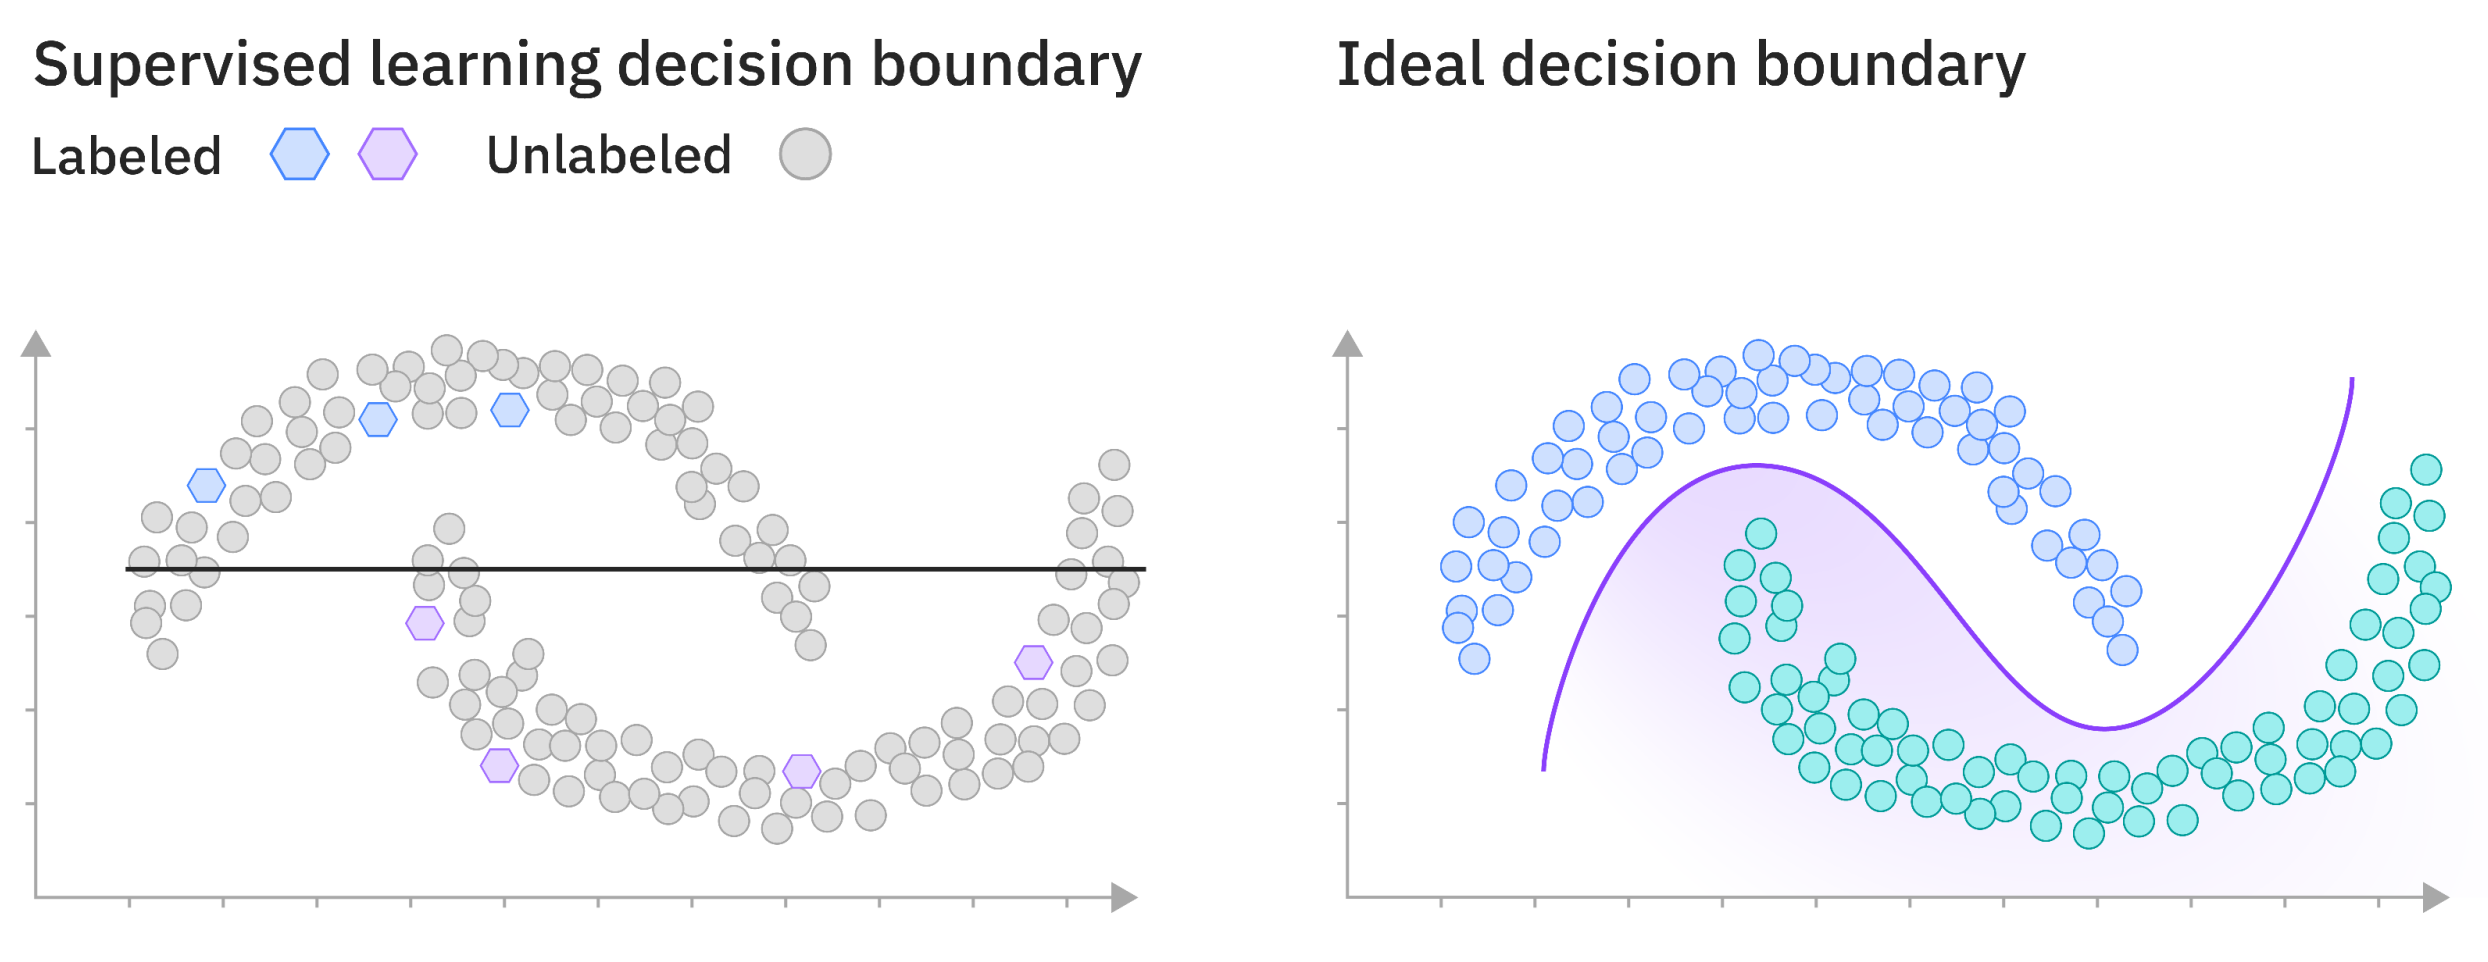
\includegraphics[width=\textwidth]{supervised}
	\caption{Using only the very limited labeled data points available, a supervised model may learn a decision boundary that will generalize poorly and be prone to misclassifying new examples. Source: \textcite{bergmann2023semi}.}
	\label{fig:supervised}
\end{figure}

In supervised pre-training, LLMs are exposed to a vast array of labeled data across various domains.
This training regime involves teaching the model to predict the correct output given an input, under the supervision of known input-output pairs.
This approach not only helps in learning general language representations but also imbues the model with domain-specific knowledge, which is particularly beneficial when the subsequent fine-tuning task is closely related to the pre-training data~\cite{phang2019sentence}.

One significant advantage of supervised pre-training is its potential to reduce the amount of labeled data required for fine-tuning on specific tasks.
By learning robust representations during pre-training, LLMs can achieve high performance on downstream tasks even with relatively smaller datasets, a concept known as transfer learning~\cite{ruder2019transfer}.
Moreover, supervised pre-training can lead to improvements in model generalization, making LLMs more adept at handling unseen data or tasks that diverge from their initial training corpus.\\

The reliance on large labeled datasets introduces concerns regarding the cost and feasibility of data annotation, especially in specialized domains where expert knowledge is required.\\
Furthermore, as shown in Figure~\ref{fig:supervised}, the risk of overfitting to the pre-training data is non-trivial, necessitating careful regularization and validation to ensure the model's generalizability~\cite{howard2018universal}.

\subsubsection{Semi-supervised pre-training}
\label{subsubsec:semi-supervised-pre-training}

Semi-supervised pre-training emerges as a compelling paradigm in the evolution of Large Language Models (LLMs), blending the strengths of supervised and unsupervised learning methodologies.
This hybrid training approach leverages a combination of labeled and unlabeled data, optimizing the utilization of available information and enhancing the model's learning efficacy and adaptability~\cite{zhu2005semi, chapelle2009semi}.

At its core, semi-supervised pre-training involves the initial training of models using a vast corpus of unlabeled data, akin to unsupervised pre-training.
This phase allows the model to capture a broad understanding of language structures and patterns.
Subsequently, the model undergoes further training or fine-tuning on a smaller labeled dataset, which instills task-specific knowledge and nuances~\cite{ruder2019transfer, yang2017transfer}.
The rationale behind this approach is to exploit the abundance of readily available unlabeled data to develop a comprehensive language model, which is then refined using the more scarce labeled data to achieve superior performance on target tasks.

Various techniques underpin semi-supervised pre-training in LLMs. One prominent method involves self-training, where the model, initially trained on labeled data, generates pseudo-labels for the unlabeled dataset.
These pseudo-labeled data points are then incorporated into further training cycles, iteratively enhancing the model's accuracy and robustness~\cite{lee2013pseudo}.

Another notable technique is the use of consistency regularization, which ensures that the model produces similar outputs for perturbed versions of the same input data, enhancing the model's stability and generalization capabilities~\cite{sajjadi2016regularization}.

Other key techniques in semi-supervised learning include transductive and inductive learning, with practical methods like label propagation and active learning aiding in leveraging unlabeled data.
These approaches are instrumental in refining the model's decision-making capabilities~\cite{bergmann2023semi}.

Transductive learning, a concept primarily attributed to \textcite{vapnik1998statistical}, focuses on predicting specific examples from the training set without attempting to generalize beyond those.
In transductive inference, the model is directly applied to the specific test set, aiming to infer the correct labels for the given unlabeled data.
The key characteristic distinguishing transductive learning from other machine learning methods is its focus on the particular sample at hand rather than on a general rule applicable to new, unseen instances.
One of the main applications of transductive learning is in the realm of support vector machines (SVMs), where it is employed to predict labels for a given, fixed set of test data, optimizing the margin not only for the training data but also for the test data, despite their labels being unknown~\cite{joachims1999transductive}.

Conversely, inductive learning aims to build a general model that predicts outcomes for new, unseen data based on the patterns learned from the training data.
Label propagation (Figure~\ref{fig:label_propagation}) is a common technique in inductive learning, where the model infers the labels of unlabeled data points based on the labels of their neighbors in the feature space.

\begin{figure}[h]
	\centering
	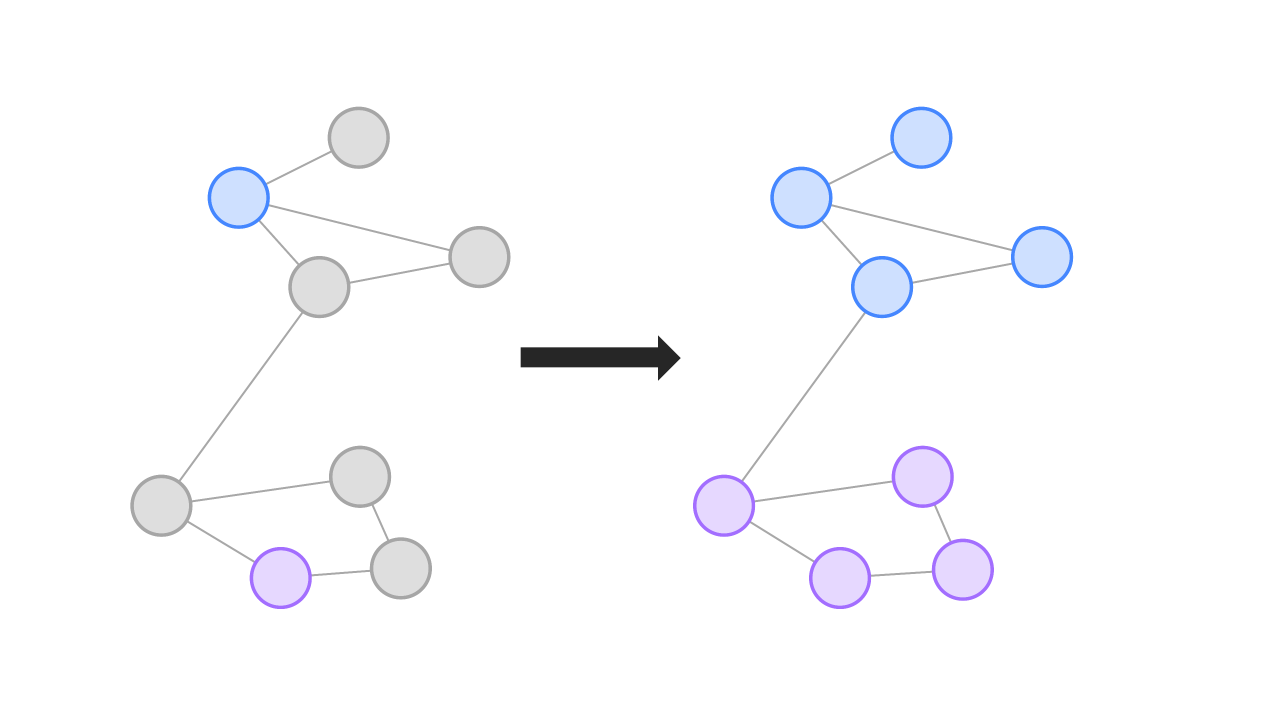
\includegraphics[width=\textwidth]{label_propagation}
	\caption{LEFT: original labeled and unlabeled data points. RIGHT: using label propagation, the unlabeled data points have been assigned pseudo-labels. Source: \textcite{bergmann2023semi}.}
	\label{fig:label_propagation}
\end{figure}

Active learning is another inductive learning method that involves iteratively selecting the most informative data points for labeling, optimizing the model's performance with minimal labeled data.
This approach is more general than transductive learning and underpins most supervised learning algorithms.
The objective here is to infer a function that can generalize well across unseen samples, not just the examples provided during the training phase.
Inductive learning is fundamental to numerous machine learning algorithms, from linear regression to deep neural networks, where the model learns an underlying function that maps input data to output predictions, with the hope that this function will perform accurately on data not present in the training set~\cite{mitchell1997machine}.

Semi-supervised approach is predicated on certain assumptions about the underlying structure and distribution of the data, which facilitate the effective integration of unlabeled data into the learning process.
\begin{itemize}
	\item \textbf{Cluster Assumption:} {The cluster assumption posits that data points within the same cluster are more likely to share a label. This assumption underpins the idea that data points in high-density regions of the input space belong to the same class, while low-density regions denote boundaries between classes~\cite{chapelle2009semi}. This principle guides the model to generalize from labeled data points to nearby unlabeled ones within the same cluster.}
	\item \textbf{Continuity Assumption:} {Also known as the smoothness assumption, this posits that if two points in the input space are close to each other, than their corresponding outputs are also likely to be similar~\cite{zhou2004learning}. In practical terms, this means that if two data points are close in the feature space, they are likely to share the same label.}
	\item \textbf{Manifold Assumption:} {The manifold assumption suggests that high-dimensional data lie on a low-dimensional manifold. This assumption implies that the data points are situated on a manifold of much lower dimensionality embedded within the higher-dimensional space, and learning can be simplified if this manifold structure is discovered and exploited~\cite{belkin2006manifold}. The manifold assumption often complements the cluster and continuity assumptions, providing a geometric interpretation of the data's distribution.}
	\item \textbf{Low-Density Separation Assumption:} {This assumption posits that the decision boundary between different classes should lie in regions of low data density~\cite{chapelle2009semi}. Essentially, it is expected that there is a natural separation or gap between classes, and the learning algorithm should prefer hypotheses that place the decision boundary in regions where few data points are present.}
\end{itemize}

\subsection{Data source}
\label{subsec:data-source}

Large Language Models (LLMs) exhibit a strong dependency on extensive, high-caliber data for pre-training, with their efficacy closely tied to the nature and preprocessing of the utilized corpora.
The main sources of data for training and evaluating LLMs can be broadly categorized into general and specialized datasets, each serving distinct purposes in enhancing the models' capabilities~\cite{survey}.\\

\begin{figure}[h]
	\centering
	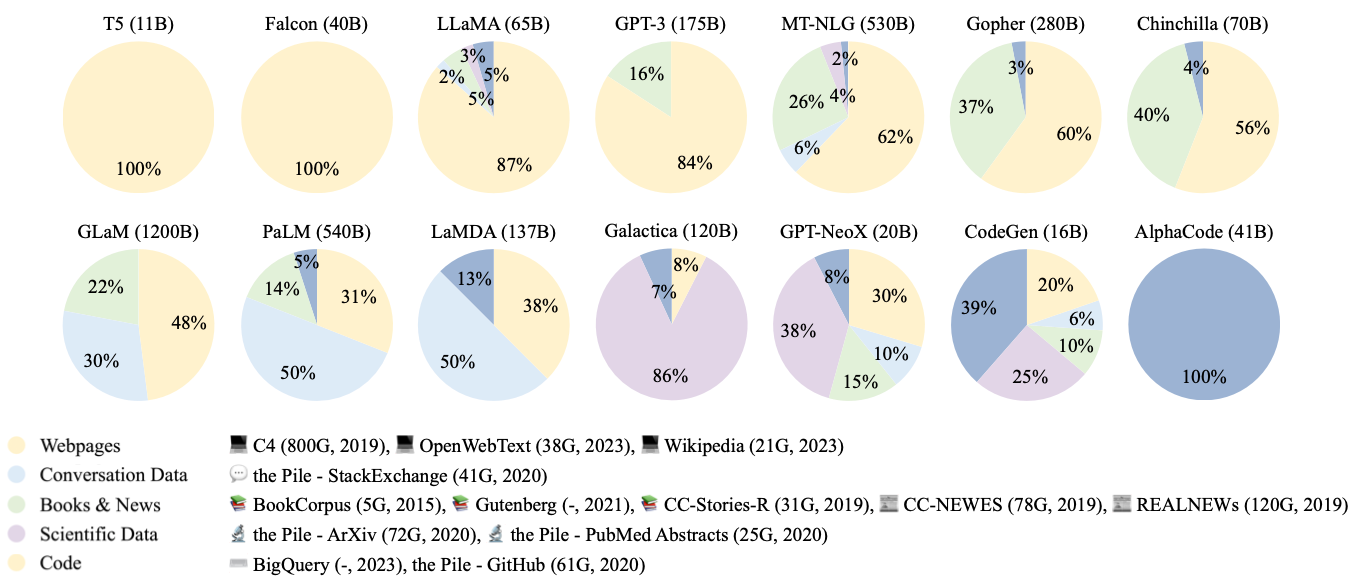
\includegraphics[width=\textwidth]{datasources}
	\caption{Commonly-used data sources for training and evaluating Large Language Models (LLMs). Source: \textcite{survey}.}
	\label{fig:data_sources}
\end{figure}

\textbf{General Data:} This category typically encompasses web content, literary works, and conversational texts, prized for their voluminous, varied, and accessible nature, thereby bolstering the language modeling and generalization prowess of LLMs. The inclusion of general data, such as web pages and books, offers a rich lexicon spanning various themes, essential for the comprehensive training of LLMs. As shown in Figure~\ref{fig:data_sources}, general purpose data are among the most commonly used general data sources for training LLMs.\\
Three important general data sources are:
\begin{itemize}
	\item \textbf{Webpages:} {Web content, extracted from the internet, is a valuable source of diverse and up-to-date text data, encompassing news articles, blog posts, and forum discussions. This data is instrumental in training LLMs to gain different linguistic knowledge and enhance generalization capabilities~\cite{brown2020language, raffel2023exploring}.
		      Crawled web data tend be a mix of high-quality and noisy text, necessitating careful preprocessing to ensure the data's quality and relevance.
	      }
	\item \textbf{Conversation text:} {
		      Conversation text, including chat logs and social media interactions, provides a rich source of informal language and colloquial expressions, enabling LLMs to capture the nuances of human communication~\cite{zhang2022opt}. This data is particularly useful for training LLMs on question answering~\cite{chowdhery2022palm} and sentiment analysis tasks~\cite{zellers2019defending}.\\
		      Conversational data often involve multiple speakers, so an effective way is to trasform the conversation in a tree structure, where the utterance is linked to the one it is replying to. The tree can be divided in multiple subtrees, each one representing a sub-conversation, which can be collected in the pre-training corpus.
		      Overtraining on conversational data can lead to the model to a performance decline, since the declarative instructions and direct interrogatives can be erroneously interpreted as the beginning of a conversation~\cite{zhang2022opt}.
	      }
	\item \textbf{Books:} {
		      Books, comprising novels, essays, and scientific literature, offer a rich source of long structured and coherent text data, enabling LLMs to learn complex language structures and thematic nuances~\cite{zhu2015aligning}. This data is instrumental in training LLMs on literary text generation tasks and enhancing their proficiency in narrative comprehension and storytelling~\cite{radford2019language}.
	      }
\end{itemize}

\textbf{Specialized Data:} Tailored to refine LLMs' proficiency in particular tasks, specialized datasets encompass multilingual text, scientific literature, and programming code.
Specialized datasets are useful to improve the specific capabilities of LLMs on downstream tasks.
Next, we introduce three kinds of specialized data.
\begin{itemize}
	\item \textbf{Multilingual text:} {
		      Multilingual text data, spanning multiple languages and dialects, is crucial for training LLMs to understand and generate text in diverse linguistic contexts~\cite{survey}. This data is instrumental in enhancing the models' cross-lingual capabilities and enabling them to perform translation tasks across different languages~\cite{survey}.
		      BLOOM~\cite{workshop2023bloom} and PaLM~\cite{chowdhery2022palm} are two models that have been trained on multilingual text data to improve their performance on cross-lingual tasks. They have impressive performances on translation, multilingual question answering, and cross-lingual summarization tasks, and they achieve comparable or superior results to models fine-tuned on specific languages.
	      }
	\item \textbf{Scientific literature:} {
		      Scientific literature, encompassing research papers, patents, and technical documents, provides a rich source of domain-specific text data, essential for training LLMs on scientific text generation and reasoning tasks~\cite{survey, taylor2022galactica, lewkowycz2022minerva}.
		      To build the scientific corpus for training LLMs, existing efforts mainly collect arXiv papers, scientific textbooks, math web-pages, and other related scientific resources.
		      Data in sceintific fields are complex, commonly including mathematical symbols and protein sequences, so specific tokenization and preprocessing techniques are required to transform these different formats of data into a unified form that can be processed by language models.
	      }
	\item \textbf{Code:} {
		      Code, encompassing source code snippets and software documentation, is a valuable source of structured text data, essential for training LLMs on code generation and code completion tasks~\cite{survey, nijkamp2022codegen}.
		      Code data is often collected from open-source repositories like GitHub and StackOverflow, and it is used to train LLMs to generate code snippets, complete code fragments, and perform code summarization tasks.
		      Recently ~\textcite{chen2021evaluating, austin2021program} have shown that models trained on code data can be used to generate code with high accuracy and efficiency, and they can be used to improve the performance of code completion tasks. Generated code can successfully pass expert-designed unit-test cases~\cite{chen2021evaluating} or solve competitive programming problems~\cite{li2022competition}.
		      In general, two types of code corpora are used: one is question answering datasets like Stack Exchange~\cite{xu2022systematic}; the second is public software repositoris like GitHub~\cite{chen2021evaluating} where code, comments and docstring are collected for utilization.
	      }
\end{itemize}

\subsubsection{Commonly-used data sources}
\label{subsubsec:commonly-used-data-sources}

The development and evaluation of Large Language Models (LLMs) rely heavily on the availability of high-quality datasets that span diverse domains and languages.
The datasets in Table~\ref{tab:table} serve as the foundation for pre-training and fine-tuning LLMs, enabling researchers to assess the models' performance on a wide range of tasks, from text generation to translation.\\

\begin{table}[h]
	\centering
	\begin{tabularx}{\textwidth}{|X|X|X|X|}
		\hline
		\textbf{Corpora}                           & \textbf{Size} & \textbf{Source} & \textbf{Update Time} \\
		\hline
		BookCorpus~\cite{zhu2015aligning}          & 5GB           & Books           & Dec-2015             \\
		Gutenberg~\cite{projectgutenberg}          & -             & Books           & Dec-2021             \\
		C4~\cite{raffel2023exploring}              & 800GB         & CommonCrawl     & Apr-2019             \\
		CC-Stories-R~\cite{trinh2018simple}        & 31GB          & CommonCrawl     & Sep-2019             \\
		CC-NEWS~\cite{liu2019roberta}              & 78GB          & CommonCrawl     & Feb-2019             \\
		REALNEWS~\cite{zellers2019defending}       & 120GB         & CommonCrawl     & Apr-2019             \\
		OpenWebText~\cite{gokaslan2019openwebtext} & 38GB          & Reddit links    & Mar-2023             \\
		Pushift.io~\cite{baumgartner2020pushshift} & 2TB           & Reddit links    & Mar-2023             \\
		Wikipedia~\cite{wikipedia}                 & 21GB          & Wikipedia       & Mar-2023             \\
		BigQuery~\cite{bigquerydataset}            & -             & Codes           & Dec-2023             \\
		the Pile~\cite{gao2021pile}                & 800GB         & Other           & Dec-2020             \\
		ROOTS~\cite{laurencon2022bigscience}       & 1.6TB         & Other           & Jun-2022             \\
		\hline
	\end{tabularx}
	\caption{Statistics of commonly-used data sources. Source: \textcite{survey}}
	\label{tab:table}
\end{table}

In this section, we will explore some of the most commonly-used data sources for training and evaluating LLMs.
Based on their content types, we categorize these corpora into six groups: Books, CommonCrawl, Reddit links, Wikipedia, Code, and others.

\begin{itemize}
	\item \textbf{Books:} {
		      BookCorpus~\cite{zhu2015aligning} and Gutenberg~\cite{projectgutenberg} are two prominent datasets that contain text from a wide range of books, spanning various genres and topics. These datasets are valuable for training LLMs on literary text and assessing their performance on text generation tasks.\\
		      BookCorpus is a dataset consisting of text from over 11,000 books (e.g., novels and biographies), while Gutenberg is a collection of over 70,000 free ebooks including novels, essays, poetry, drama, history, science, philosophy, and other types of works in the public domain.\\
		      BookCorpus is commonly used in previous small-scale models (e.g., GPT~\cite{radford2018improving} and GPT-2~\cite{radford2019language}), while Gutenberg is used in more recent large-scale models (i.e., LLaMa~\cite{touvron2023llama}).\\
		      Book1 and Book2 used in GPT-3~\cite{brown2020language} are much larger than BookCorpus, but they have not been publicly released.
	      }
	\item \textbf{CommonCrawl:} {
		      CommonCrawl~\cite{commoncrawl} is a vast web corpus that contains data from billions of web pages, covering diverse topics and languages. Due to noise and redundancy in the data, researchers often extract subsets of CommonCrawl for training LLMs. The main subsets used for training LLMs are C4\footnote{Colossal Clean Crawled Corpus}~\cite{raffel2023exploring}, CC-Stories-R~\cite{trinh2018simple}, CC-NEWS~\cite{liu2019roberta}, and REALNEWS~\cite{zellers2019defending}.\\
	      }
	\item \textbf{Reddit links:} {
		      Reddit is a social media platform where users can submit links and posts and "upvotes" or "downvote" them. Posts with high number of "upvotes" are often considered useful, and can be used to create high-quality datasets.
		      OpenWebText~\cite{gokaslan2019openwebtext} and Pushshift.io~\cite{baumgartner2020pushshift} are datasets that contain text data extracted from Reddit. These datasets are useful for training LLMs on social media text and assessing their performance on text generation and sentiment analysis tasks.
	      }
	\item \textbf{Wikipedia:} {
		      Wikipedia~\cite{wikipedia} is a widely-used dataset that contains text from articles on various topics. It's an online encyclopedia with a large volume of high-quality articles. Most of these articles are composed in an expository style of writing (with supporting references), covering a wide range of languages and fields.
		      Typically, the English-only filtered versions of Wikipedia are widely used in most LLMs (e.g., GPT-3~\cite{brown2020language}, and LLaMA~\cite{touvron2023llama}).
		      Wikipedia is available in multiple languages, so it can be used in multilingual settings.
	      }
	\item \textbf{Code:} {
		      Two major sources are GitHub, for open-source licensed code, and StackOverflow, for code-related question-answering platforms.\\
		      Google has publicly released BigQuery~\cite{bigquerydataset}, a dataset that contains code snippets from various programming languages. This dataset is useful for training LLMs (i.e., CodeGen~\cite{nijkamp2022codegen}) on code text and assessing their performance on code generation and code completion tasks.
	      }
	\item \textbf{Others:} {
		      The Pile~\cite{gao2021pile} and ROOTS~\cite{laurencon2022bigscience} are datasets that contain text data from various sources, such as books, articles, and websites.\\
		      The Pile contains 800GB of data from multiple sources, including books, websites, codes, scientific papers, and social media platforms. It's widely used in training LLMs with different size (e.g., CodeGen(16B)~\cite{nijkamp2022codegen} and Megatron-Turing NLG(530B)~\cite{smith2022deepspeed}).\\
		      ROOTS is composed of various smaller datasets (totally 1.61 TB of text) in 59 different languages (containing natural languages and programming languages). It's been used for training BLOOM~\cite{workshop2023bloom}.
	      }
\end{itemize}

In practice, a mixture of these datasets is often used to train LLMs, as they provide a diverse range of text data (Figure~\ref{fig:data_sources}).
The choice of datasets depends on the specific task and domain of interest, as well as the computational resources available for training the model.
Furthermore, to train LLMs that are adaptative to specific tasks or domains, is also important to consider the data sources that are relevant to them.\\

\subsection{Data preprocessing}
\label{subsec:data-preprocessing}

After collecting the data, the next step is to preprocess it to ensure that it is clean, consistent, and ready for training Large Language Models (LLMs) removing noise and irrelevant, or potentially toxic information~\cite{chowdhery2022palm, rae2021scaling, longpre2023pretrainer}.
In \textcite{chen2023datajuicer} the authors propose a new data preprocessing system, DataJuicer, that can be used to improve quality of the processed data.\\
A typical pipeline for data preprocessing involves several steps, as shown in Figure~\ref{fig:preprocessing}:

\begin{figure}[H]
	\centering
	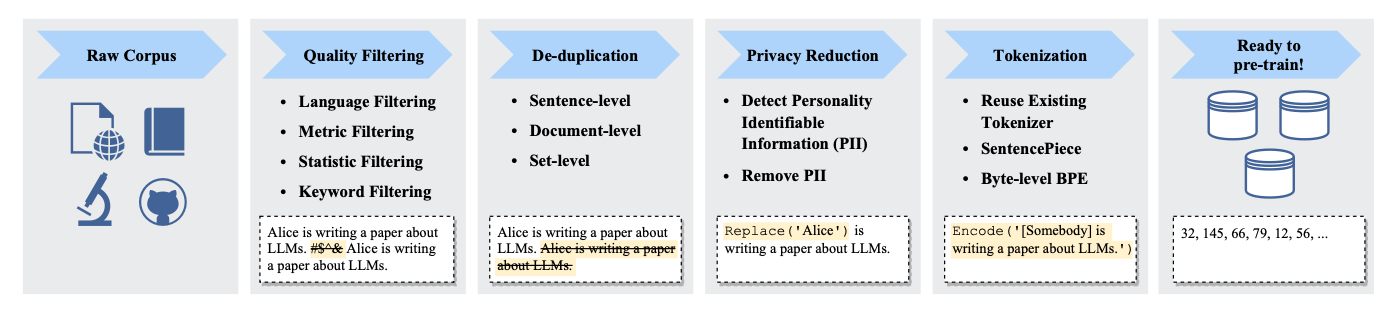
\includegraphics[width=\textwidth]{preprocessing}
	\caption{Common data preprocessing steps for training Large Language Models (LLMs). Source: \textcite{survey}.}
	\label{fig:preprocessing}
\end{figure}

\textbf{Quality Filtering.}
The first step in data preprocessing is quality filtering, where the data is cleaned to remove irrelevant or low-quality content.
Existing works mainly adopt two strategies for quality filtering: classifier-based and heuristic-based filtering.

The former approach involves training a classifier to distinguish between high-quality and low-quality data, using well-curated data (e.g., Wikipedia pages) as positive examples and noisy data (e.g., spam or irrelevant content) as negative examples.
\textcite{rae2021scaling, du2022glam} find that classifier-based filtering may remove high-quality data in dialect, colloquial, and sociolectal\footnote{In sociolinguistics, a sociolect is a form of language or a set of lexical items used by a socioeconomic class, profession, age group, or other social group. Sociolects involve both passive acquisition of particular communicative practices through association with a local community, as well as active learning and choice among speech or writing forms to demonstrate identification with particular groups. Source: \textcite{wikipedia}} languages, which potentially leads to bias in the pre-training data and diminishes the corpus diversity.\\
Heuristic-based filtering, on the other hand, involves setting predefined rules to identify and remove noisy data~\cite{workshop2023bloom, rae2021scaling}.
The set of rules can be summarized as follows:
\begin{itemize}
	\item \textit{Language based filtering}. {Remove data that is not in the target language.}
	\item \textit{Metric based filtering}. {Remove data that does not meet certain quality metrics, e.g., perplexity, readability, or coherence.
	      Perplexity (PPL) is one of the most common metrics for evaluating language models.
	      This metric applies specifically to classical language models (sometimes called autoregressive or causal language models) and is not well-defined for masked language models like BERT~\cite{devlin2019bert}.
	      Perplexity is defined as the exponential average negative log-likelihood of a sequence.\\
	      If we have a tokenized sequence \(X = x_1, x_2, \ldots, x_t\), the perplexity of the sequence is defined as:
	      \begin{equation}
		      PPL(X) = \exp \left\{ -\frac{1}{t} \sum_{i}^{t} \log p_{\theta}(x_i | x_{<i}) \right\}
		      \label{eq:equation_perplexity}
	      \end{equation}
	      where \(\log p_{\theta}(x_i | x_{<i})\) is the log-likelihood of the token \(x_i\) given the previous tokens \(x_{<i}\) in the sequence.
	      Intuitively, it can be thought of as an evaluation of the model’s ability to predict uniformly among the set of specified tokens in a corpus\footnote{This means that the tokenization procedure has a direct impact on a model’s perplexity which should always be taken into consideration when comparing different models.}~\cite{huggingface2023perplexity}.
	      }
	\item \textit{Statistic based filtering}. {Statistical features like punctuation distribution, symbol-to-word ratio, and sentence length can be used to filter out low-quality data.
	      }
	\item \textit{Keyword based filtering}. {Remove data that contains specific keywords that are noisy, irrelevant or toxic like HTML tags, URLs, boilerplate text, or offensive language.}
\end{itemize}

\textbf{Deduplication.}
The next step in data preprocessing is deduplication, where duplicate data  are removed to reduce redundancy and improve the diversity of the training data.
Moreover, \textcite{hernandez2022scaling} found that duplication may cause instability in the training process, leading to overfitting and poor generalization performance.
Therefore, deduplication is essential to ensure that the model is exposed to a diverse range of text data during training.

It can be done at various granularity, such as at the document level, paragraph level, or sentence level.
Low-quality sentences that contains repeated words or phrases can be removed to improve the quality of the data.
At document level, the deduplication can be done by computing overlap ratio of surface features (e.g., words and n-grams overlap) between documents, and removing the duplicates that contains similar contents~\cite{touvron2023llama,rae2021scaling,workshop2023bloom,lee2022deduplicating}.
To avoid the contamination problem, the deduplication process should be done before the data is split into training, validation, and test sets~\cite{chowdhery2022palm}.
\textcite{chowdhery2022palm} and \textcite{carlini2022quantifying} have shown that the three deduplication strategies should be used in conjunction to improve the training of LLMs.

\textbf{Privacy reduction.}
Privacy reduction is another important step in data preprocessing, especially when dealing with sensitive or personal information.
Since data is often collected from web and contains user-generated content, the risk of privacy breaching is high~\cite{carlini2021extracting}.
This step involves anonymizing or obfuscating sensitive data to protect the privacy of individuals.
Common techniques for privacy reduction include masking personally identifiable information (PII), such as names, addresses, and phone numbers, and replacing them with generic placeholders or tokens~\cite{laurencon2022bigscience}.\\
Privacy attacks to LLMs can be attributed to presence of duplicated PII data in the pre-training, which can be used to extract the original PII data~\cite{lee2022deduplicating}.
Therefore, de-duplication can also reduce privacy risks to some extent.

\textbf{Tokenization.}
Tokenization is a crucial step in data preprocessing, where the text data is converted into tokens that can be processed by the model.
The choice of tokenization method can have a significant impact on the model's performance, as different tokenization strategies can affect the model's ability to capture the underlying structure of the language.

Common tokenization techniques include word-based tokenization, subword-based tokenization, and character-based tokenization.
Word-based tokenization splits the text into individual words, while subword-based tokenization breaks down the text into subword units, such as prefixes, suffixes, and roots.
Character-based tokenization, on the other hand, tokenizes the text into individual characters.
Word-based tokenization is the predominant method used in traditional NLP research~\cite{lafferty2001conditional}.

However, word-based tokenization can be problematic for languages with complex morphology or limited vocabulary, as it may result in a large vocabulary size and sparse data representation.
In some other languages, like Chinese, Japanese, and Korean, word-based tokenization is not suitable because these languages do not have explicit word boundaries\footnote{It means that it can yield different segmentation results for the same input.}.
Thus, several neural network-based models employed subword-based tokenization, such as Byte Pair Encoding (BPE)~\cite{sennrich2016neural}, Unigram~\cite{kudo2018sentencepiece}, and WordPiece~\cite{wu2016google}, to address these challenges.

Byte Pair Encoding (BPE) is a type of data compression technique that has been effectively adapted for natural language processing tasks, particularly in the domain of tokenization for large language models (LLMs).
The BPE algorithm operates by iteratively merging the most frequent pair of bytes (or characters in the context of text) in a given dataset into a single, new byte (or character), and it repeats this process until a specified number of merges has been reached or another stopping criterion has been met.
The application of BPE in the field of NLP was popularized by \textcite{sennrich2016neural} in the context of neural machine translation.
They demonstrated that using BPE allowed for efficient handling of rare and unknown words, which are commonplace in languages with rich morphology or in specialized vocabularies, such as scientific texts or code.
By splitting words into subword units, BPE provides a balance between the granularity of characters and the semantic units of full words, enabling models to represent a wide vocabulary with a limited set of tokens.
BPE has been fundamental in the architecture of influential language models, such as OpenAI's GPT series, BART and LLaMA\@.

WordPiece tokenization is a tokenization method that segments text into subword units, allowing for a balance between the flexibility of character-based models and the efficiency of word-based models.
Originating from speech processing~\cite{wu2016google}, this method has found significant application in natural language processing, particularly within neural network-based models such as BERT and its variants.
In WordPiece tokenization, a base vocabulary is first constructed with individual characters, and then more frequent and meaningful sub-word units are incrementally added.
This construction process is guided by a criterion that aims to maximize the language model likelihood on a training corpus, thus ensuring that the resulting tokens are optimal representations for the given data.
The WordPiece algorithm iteratively merges the most frequently co-occurring pairs of tokens to form new sub-word units until a specified vocabulary size is reached.
This tokenization strategy has shown effectiveness in reducing out-of-vocabulary issues, as the model can fall back on smaller sub-word units when encountering unfamiliar words.
Moreover, by capturing sub-word regularities, WordPiece facilitates the learning of meaningful representations for morphologically rich languages within large language models.
This is particularly advantageous for handling agglutinative languages, where words often comprise a series of affixed morphemes\footnote{
	Agglutinative languages are a type of morphological linguistic classification in which words are formed through the linear addition of discrete units, each of which carries a specific grammatical meaning. These discrete units are known as morphemes, which are the smallest grammatical units in a language. In agglutinative languages, morphemes are concatenated in a way that each morpheme represents a single grammatical function, such as tense, number, case, or aspect.
	For example, in Turkish -- an agglutinative language -- a single word can be made up of a base or root word with several affixes attached to it to modify its meaning. These affixes remain relatively invariant; they don’t undergo significant changes in form when they’re combined with other morphemes. Here’s an illustrative example from Turkish:\\
	"ev" means "house"\\
	"evler" means "houses" (plural)\\
	"evlerim" means "my houses" (possessive plural)\\
	Each suffix attached to "ev" is a separate morpheme that changes the meaning of the word, indicating plurality and possession without ambiguity.
	This is in contrast to fusional languages, where a single affix can represent multiple grammatical categories, or isolating languages, where words generally do not change form at all, and grammatical relations are indicated by word order or separate words.
}.

Unigram tokenization is a statistical method that employs an unigram language model for the probabilistic segmentation of text into tokens.
This technique, standing in contrast to the deterministic nature of Byte Pair Encoding, involves constructing a unigram model from a large initial vocabulary and iteratively refining it to maximize the likelihood of the observed corpus~\cite{kudo2018sentencepiece}.
The essence of Unigram tokenization lies in its iterative pruning process, wherein less probable tokens are systematically eliminated from the vocabulary.
To estimate the unigram language model, it adopts an expectation–maximization (EM) algorithm: at each iteration, it first finds the currently optimal tokenization of words based on the old language model, and then re-estimate the probabilities of unigrams to update the language model.
During this procedure, dynamic programming algorithms (i.e., the Viterbi algorithm) are used to efficiently find the optimal decomposition way of a word given the language model\cite{survey}.
This probabilistic approach is adept at handling the linguistic complexities and variations found across different languages and domains.
It particularly excels in the context of language models that require a nuanced understanding of morphological structures and sub-word variations.
Unigram tokenization has been pivotal in the development of the SentencePiece~\cite{kudo2018sentencepiece} tokenization library, which is renowned for its application in T5 and mBART\@.
The adaptability and language-agnostic properties of Unigram tokenization make it a preferred choice for LLMs tasked with processing multilingual data~\cite{kudo2018sentencepiece}.

\section{Adaptation of Large Language Models}
\label{sec:adaptation-of-llms}

The adaptation of Large Language Models (LLMs) is a critical aspect of their deployment in real-world applications, as it enables the models to be fine-tuned on specific tasks or domains after pre-training, enhancing their performance minimizing loss of  generalization capabilities.
Adaptation can be achieved through various techniques, such as instruction tuning and alignment tuning, which allow LLMs to enhance (or unlock) theirs abilities and align their behaviours with human values or preferences~\cite{survey}.

\begin{table}[htbp]
	\centering
	\caption{A detailed list of available collections for instruction tuning.}
	\label{tab:instruction_tuning}
	\begin{tabularx}{\textwidth}{|X|X|X|X|}
		\hline
		\textbf{Categories} & \textbf{Collections}                        & \textbf{Time} & \textbf{\#Examples} \\
		\hline
		Task                & Nat. Inst. \cite{mishra2022crosstask}       & Apr-2021      & 193K                \\
		                    & FLAN~\cite{wei2022fine}                     & Sep-2021      & 4.4M                \\
		                    & P3~\cite{bach2022promptsource}              & Oct-2021      & 12.1M               \\
		                    & Super Nat. Inst. \cite{wang2022super}       & Apr-2022      & 5M                  \\
		                    & MVPCorpus~\cite{tang2022mvp}                & Jun-2022      & 41M                 \\
		                    & xP3~\cite{muennighoff2022crosslingual}      & Nov-2022      & 81M                 \\
		                    & OIG~\cite{vaswani2023attention}             & Mar-2023      & 43M                 \\
		\hline
		Chat                & HH-RLHF~\cite{bai2022training}              & Apr-2022      & 160K                \\
		                    & HC3~\cite{guo2023close}                     & Jan-2023      & 87K                 \\
		                    & ShareGPT~\cite{devlin2019bert}              & Mar-2023      & 90K                 \\
		                    & Dolly~\cite{lewis2020bart}                  & Apr-2023      & 15K                 \\
		                    & OpenAssistant~\cite{koepf2023openassistant} & Apr-2023      & 161K                \\
		\hline
		Synthetic           & Self-Instruct~\cite{wang2022selfinstruct}   & Dec-2022      & 82K                 \\
		                    & Alpaca~\cite{taori2023stanford}             & Mar-2023      & 52K                 \\
		                    & Guanaco~\cite{fedus2021switch}              & Mar-2023      & 535K                \\
		                    & Baize~\cite{xu2023baize}                    & Apr-2023      & 158K                \\
		                    & BELLE~\cite{ji2023towards}                  & Apr-2023      & 1.5M                \\
		\hline
	\end{tabularx}
\end{table}

\subsection{Instruction Tuning}
\label{subsec:instruction-tuning}

Instruction tuning is a technique that leverages natural language instructions to fine-tune pre-trained LLMs~\cite{wei2022fine}, which is highly related to supervised fine-tuning~\cite{ouyang2022training} and multi-task prompted training~\cite{sanhetal2022multitask}.
Instruction tuning enhances LLMs by refining their ability to follow and comprehend natural language instructions.
Unlike traditional fine-tuning, which adapts models to specific tasks, instruction tuning employs a more generalized approach that broadens the model's utility across a variety of tasks through an "instruction-following" paradigm (Figure~\ref{fig:instruction-tuning}).

\begin{figure}[h!]
	\centering
	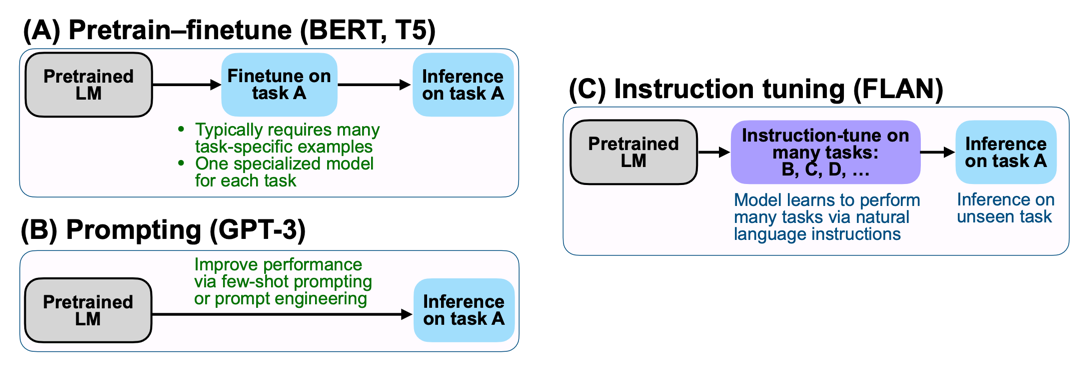
\includegraphics[width=\textwidth]{instruction-tuning}
	\caption{Overview of instruction tuning. Source: \textcite{survey}.}
	\label{fig:instruction-tuning}
\end{figure}

FLAN\footnote{Finetuned LAnguage Net, a 137B parameter pretrained language model and instruction tune it on over 60 NLP datasets verbalized via natural language instruction templates}~\cite{wei2022fine} is noted for substantially improving zero-shot learning capabilities when compared to traditional models like GPT-3~\cite{brown2020language} (Figure~\ref{fig:instruction-tuning-comparison}).

\begin{figure}[h!]
	\centering
	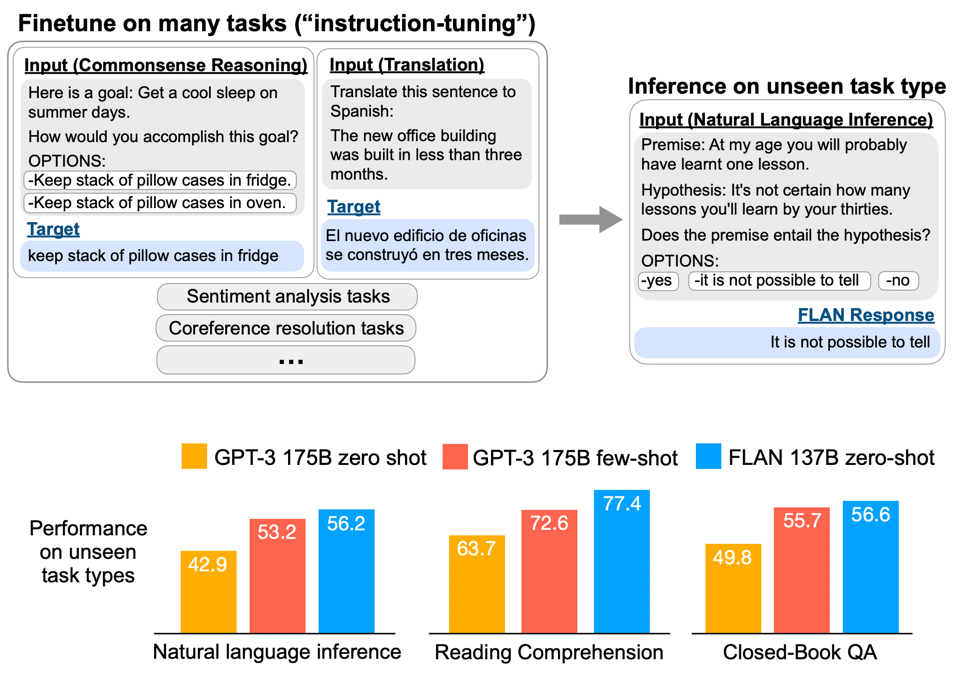
\includegraphics[width=\textwidth]{instruction-tuning-comparison}
	\caption{Top: overview of instruction tuning and FLAN. Instruction tuning finetunes a pretrained language model on a mixture of tasks phrased as instructions. Evaluation on unseen task type at inference time (i.e., evaluate the model on natural language inference (NLI) when no NLI tasks were seen during instruction tuning).\\
		Bottom: performance of zero-shot FLAN, compared with zero-shot and few-shot GPT-3, on three unseen task types where instruction tuning improved performance substantially out of ten evaluated. NLI datasets: ANLI R1–R3, CB, RTE. Reading comprehension datasets: BoolQ, MultiRC, OBQA. Closed-book QA datasets: ARC-easy, ARC-challenge, NQ, TriviaQA.
		Source: \textcite{wei2022fine}.}
	\label{fig:instruction-tuning-comparison}
\end{figure}

\textcite{chung2022scaling} have shown instruction-tuned (Figure~\ref{fig:instruction-finetuning}) PaLM\footnote{Also called Flan-PaLM 540B-parameter model} enhance model performance on various tasks (i.e., MMLU, BBH, TyDiQA and MGSM) when the model size is at least 62B, though a much smaller size might suffice for some specific tasks (e.g., MMLU).

\begin{figure}[h!]
	\centering
	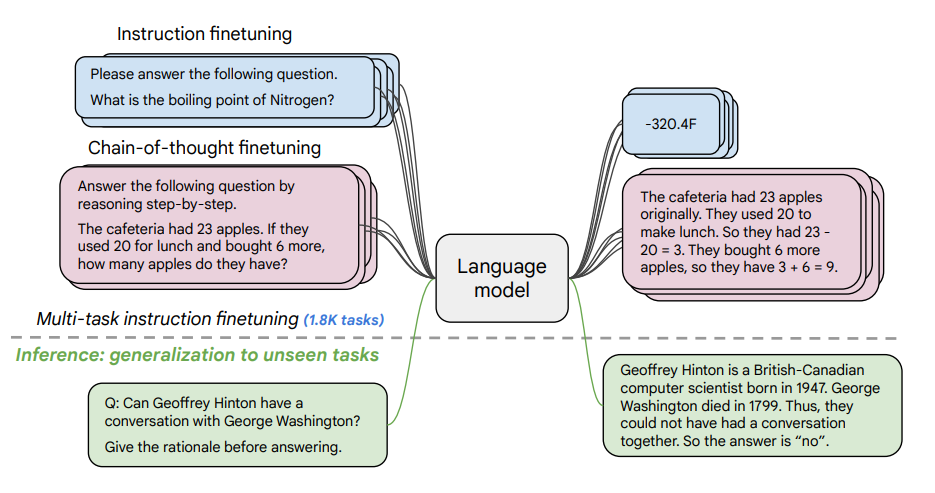
\includegraphics[width=\textwidth]{instruction-finetuning}
	\caption{Overview of FLAN instruction tuning with and without exemplars (i.e., zero-shot and few-shots) and with and without CoT. Following evaluation on unseen tasks. Source: \textcite{chung2022scaling}.}
	\label{fig:instruction-finetuning}
\end{figure}

Instruction tuning has been widely applied also in other models like Instruct-GPT~\cite{ouyang2022training} and GPT-4~\cite{radford2023gpt4}.
Other experiments in \textcite{wei2022fine} have shown that instruction tuning of LaMDA-PT started to significantly improve performance on zero-shot tasks when the model size is at least 68B\@.

Let's have a look at the construction of instruction-formatted instances, which are essential for instruction tuning.
Generally, an instruction-formatted instance consists of a task description (called an \textit{instruction}) and a set of input-output examples, optionally followed by a small number of demonstrations.
There are three main approaches to construct instruction-formatted instances: formatting task datasets, formatting daily dialogues, and formatting synthetic data as represented in Figure~\ref{fig:instruction-formatted-instances}.

\begin{figure}[h!]
	\centering
	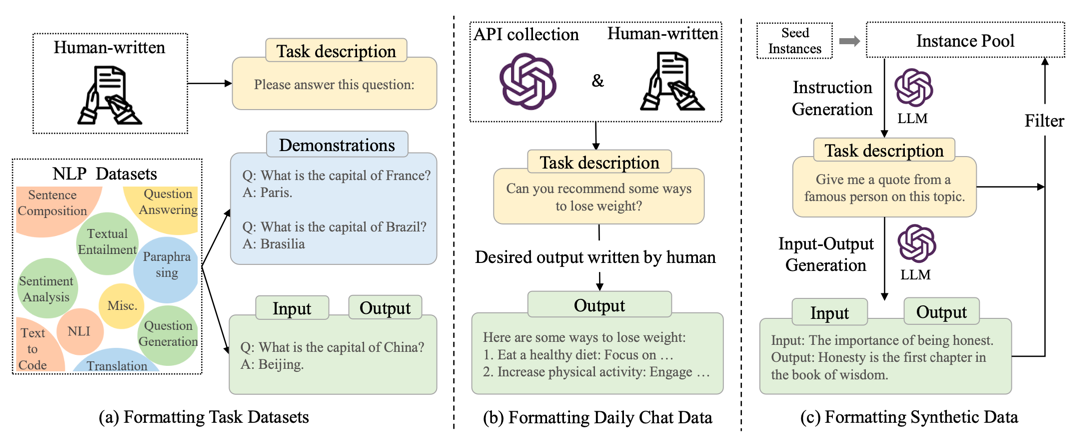
\includegraphics[width=\textwidth]{instruction-formatted-instances}
	\caption{Three main approaches to construct instruction-formatted instances. Source: \textcite{survey}.}
	\label{fig:instruction-formatted-instances}
\end{figure}

Historically, datasets encompassing various tasks like text summarization, classification, and translation were used to create multi-task training datasets~\cite{tang2022mvp,liu2019multi,aghajanyan2021muppet}.
These datasets have become crucial for instruction tuning, particularly when formatted with natural language descriptions that clarify the task objectives to the LLMs. This augmentation helps the models understand and execute the tasks more effectively~\cite{sanhetal2022multitask,ouyang2022training,wei2022fine, wang2022super}.
For instance, each example in a question-answering dataset might be supplemented with a directive like "Please answer this question" which guides the LLM in its response generation.
The effectiveness of such instruction tuning is evident as LLMs demonstrate improved generalization to unfamiliar tasks when trained with these enriched datasets~\cite{wei2022fine}.
The importance of these instructions is underscored by the observed decline in performance when task descriptions are omitted from training.

PromptSource~\cite{bach2022promptsource}, a crowd-sourcing platform, has been proposed to aid in the creation, sharing, and verification of task descriptions for datasets.
This platform enhances the utility of instruction tuning by ensuring a rich variety of well-defined task descriptions.
Several studies~\cite{sanhetal2022multitask, tang2022mvp, longpre2023flan} also tried to invert the input-output pairs of existing instances to create new instances using specially designed task descriptions (e.g., "Please generate a question given this answer").

Talking about formatting daily chat data, Instruct-GPT has been fine-tuned using real user queries submitted to the OpenAI API to fill the significant gap in the data used for training models -- most training instances come from public NLP datasets that often lack instructional diversity and do not align well with actual human needs.
This approach helps to harness the model's capability to follow instructions effectively.
To further enhance task diversity and real-life applicability, human labelers are employed to create instructions for a variety of tasks including open-ended generation, open question answering, brainstorming, and casual chatting.
Another set of labelers then provides responses to these instructions, which are used as training outputs.
This method not only enriches the training data but also aligns the model's responses more closely with human-like conversational patterns.
InstructGPT also employs these real-world tasks formatted in natural language for alignment tuning (see Section~\ref{subsec:alignment-tuning}).
GPT-4 extends this approach by specifically designing potentially high-risk instructions and guided the model to reject these instructions through supervised fine-tuning for safety concerns.
Recent efforts have also focused on collecting user chat requests as input data, with models like ChatGPT or GPT-4 generating the responses.
A notable dataset in this realm is the conversational data from ShareGPT, which provides a rich source of real-world interactions for training and refining the performance of LLMs.

Semi-automated methods~\cite{wang2022selfinstruct} for generating synthetic data have also been explored to create instruction-formatted instances, which helps alleviate the need for extensive human annotation and manual data collection.
One such method is the Self-Instruct approach, which efficiently utilizes a relatively small initial dataset.
With the Self-Instruct method, only about 100 examples are required to start the data augmentation process (Figure~\ref{fig:instruction-formatted-instances}c).
From this initial task pool, a few instances are selected randomly and used as demonstrations for an LLM. The model is then prompted to generate new task descriptions along with corresponding input-output pairs.
This process not only expands the dataset but also ensures a variety of training examples by incorporating a diversity and quality check before adding the newly synthesized instances back into the task pool.
This synthetic approach to data generation is portrayed as both cost-effective and efficient, providing a scalable solution for enriching training datasets for LLMs. It leverages the generative capabilities of LLMs to create diverse and relevant training materials, thereby enhancing the training process without the usual resource-intensive demands of manual data creation.
Instruction tuning not only improves zero-shot learning but also establishes new benchmarks in few-shot learning scenarios.
The improvement is attributed to the instruction tuning across diverse datasets which likely provides a richer context for model adaptation~\cite{wei2022fine}.
The idea is that by using supervision to teach a model to perform tasks described via instructions, the model will learn to follow instructions and do so even for unseen tasks.

Two essentials factors for instance construction are:
\begin{itemize}
	\item \textbf{Scaling the instructions.} {Increasing the number of tasks within training data can significantly improve the generalization ability of LLMs, as evidenced by~\textcite{wei2022fine, sanh2021distilbert, chowdhery2022palm}. The performance of LLMs typically increases with the number of tasks but plateaus after reaching a saturation point~\cite{raffel2023exploring, chowdhery2022palm}. It is suggested that beyond a certain threshold, additional tasks do not contribute to performance gains~\cite{raffel2023exploring}. The diversity in task descriptions, including variations in length, structure, and creativity, is beneficial~\cite{wei2022fine}. However, increasing the number of instances per task might lead to overfitting if the numbers are excessively high~\cite{chowdhery2022palm, chen2023maybe}.}
	\item \textbf{Formatting design.} {
		      The way instructions are formatted also plays a crucial role in the generalization performance of LLMs~\cite{chowdhery2022palm}. Task descriptions, supplemented by optional demonstrations, form the core through which LLMs grasp the tasks~\cite{chowdhery2022palm}. Utilizing a suitable number of exemplars as demonstrations can notably enhance performance and reduce the model's sensitivity to instruction nuances~\cite{sanh2021distilbert, raffel2023exploring}. However, including additional elements like prohibitions, reasons, or suggestions within instructions may not effectively impact or might even negatively affect LLM performance~\cite{chowdhery2022palm, mishra2022crosstask}. Recently, some studies suggest incorporating chain-of-thought (CoT) examples in datasets that require step-by-step reasoning, which has proven effective across a variety of reasoning tasks~\cite{raffel2023exploring, iyer2022opt}.
	      }
\end{itemize}

Instruction tuning is often more efficient since only moderate number of instances are needed for training.
Since instruction tuning can be considered as a supervised training process, its optimization is different from pre-training in several aspects~\cite{chung2022scaling}, such as the training objective (i.e., sequence-to-sequence loss) and optimization
configuration (e.g., smaller batch size and learning rate), which require special attention in practice.

Balancing the proportion of different tasks during fine-tuning is crucial.
A commonly used method is the examples-proportional mixing strategy~\cite{raffel2023exploring}, ensuring that no single dataset overwhelms the training process~\cite{raffel2023exploring, wei2022fine}.
Additionally, setting a maximum cap on the number of examples from any dataset helps maintain this balance~\cite{raffel2023exploring, wei2022fine}.

To enhance the stability and effectiveness of instruction tuning, integrating pre-training data into the tuning process is beneficial, serving as regularization~\cite{wei2022fine}.
Some models, such as GLM-130B and Galactica, start with a mix of pre-training and instruction-tuned data, effectively combining the strengths of both pre-training and instruction tuning~\cite{chowdhery2022palm, lewis2021paLM}.

A strategic approach involves multiple stages of tuning, starting with extensive task-specific data and followed by less frequent types such as daily chat instructions, to avoid the forgetting of previously learned tasks~\cite{raffel2023exploring}.

Some additional strategies to improve the instruction tuning process include:
\begin{itemize}
	\item \textbf{Efficient training for multi-turn chat data.} {Given a multiturn chat\footnote{The conversation between a user and a bot} dataset, each conversation can be split into multiple context-response pairs for training: the model is fine-tuned to generate responses based on the corresponding context for all splits. To save computational resources, \textcite{chiang2023vicuna} propose a method that fine-tunes the model on the whole conversation, but relies on a loss mask that only computes the loss on the responses of the chatbot for training.
	      }
	\item \textbf{Filtering low-quality instructions using LLMs.} {Filtering out low-quality instructions through advanced LLMs helps maintain high training standards and reduces unnecessary computational expenses~\cite{wei2022fine}.}
	\item \textbf{Establishing self-identification for LLM.} {In real world applications, it is important for LLMs to be able to identify themselves when asked. To achieve this, models like GPT-4 are trained to recognize and respond to self-identification instructions~\cite{radford2023gpt4}.
	      }
	\item \textbf{Concatenate multiple examples to approach max length.} {
		      To handle variable-length sequences during training, it is common practice to introduce padding tokens to ensure uniform sequence lengths. However, this approach can lead to inefficient use of the model's capacity, as the padding tokens do not contribute to the learning process. By concatenating multiple examples to approach the maximum sequence length, the model can process more information in each training step, thereby enhancing the training efficiency and performance~\cite{krell2021efficient}.
	      }
	\item \textbf{Evaluate the quality of instructions.}{
		      \textcite{cao2023instruction} introduced \textsc{InstructMining} to autonomously select premium instruction-following data for finetuning LLMs by employing a combination of data mining techniques and performance evaluation strategies.
		      The quality of instruction data is primarily assessed through its impact on model performance, quantified by the inference loss of a finetuned model on an evaluation dataset. \textsc{InstructMining} correlates the values of the natural language indicators\footnote{Some of the indicators include:
			      \begin{itemize}
				      \item Input and output length
				      \item Reward model scores
				      \item Perplexity
				      \item Measures of Textual Lexical Diversity (MTLD)
				      \item Approximate distance to nearest neighbors in embedding space
				      \item Scores for naturalness, coherence, and understandability from models like UniEval
			      \end{itemize}
		      }
		      with the inference loss, creating a predictive model that estimates data quality based on these indicators.
		      To identify the most effective subset of data for finetuning, \textsc{InstructMining} integrates an optimization technique called \textsc{BlendSearch}. This method helps in determining the optimal size and composition of the data subset that leads to the best finetuning outcomes. \textsc{BlendSearch} combines global and local search strategies to efficiently explore the complex search space, focusing on minimizing the model’s inference loss on a high-quality evaluation set.
		      \textcite{cao2023instruction} also accounts for the double descent phenomenon observed in model training, where increasing the dataset size initially improves performance up to a point, after which performance declines before potentially improving again as more data is added. This observation guides the selection process to focus on an optimal point that balances data quality and quantity, improving model performance efficiently.
	      }
	\item \textbf{Rewriting instructions into more complex ones.} {
		      \textcite{xu2023wizardlm} introduces an innovative method, termed "Evol-Instruct", which significantly enhances the instruction-following capabilities and overall performance of large language models (LLMs). It is a systematic approach for automatically generating complex instruction data using LLMs instead of human input. This method involves iterative evolution and refinement of initial, simpler instructions into more complex and diverse variants. These evolved instructions are then used to fine-tune LLMs, specifically targeting their ability to understand and execute more complex tasks effectively. Starting with a basic set of instructions, Evol-Instruct employs a two-pronged strategy -- In-Depth Evolving and In-Breadth Evolving.

		      In-Depth Evolving enhances the complexity and depth of instructions by adding constraints, increasing reasoning demands, or introducing more detailed contexts.
		      In-Breadth Evolving expands the variety and coverage of topics and skills addressed by the instructions, aiming to fill gaps in the LLM’s training data and increase its general robustness across different types of tasks.

		      Throughout the evolution process, ineffective or poorly structured instructions are filtered out to ensure only high-quality data is used for model training. This step is crucial for maintaining the integrity and effectiveness of the training dataset.
		      The process repeats several cycles, allowing the system to gradually refine the instruction set to maximize complexity and utility, while ensuring the instructions remain understandable and executable by the LLM.
		      By training with the complex instructions generated by Evol-Instruct, LLMs like the WizardLM demonstrate significant improvements in several key areas:
		      \begin{itemize}
			      \item Enhanced Generalization: The model becomes capable of handling a wider variety of tasks beyond the scope of its original training data.
			      \item Improved Complexity Handling: The LLM shows better performance in understanding and executing tasks that require higher levels of reasoning or multiple steps to complete.
			      \item Competitive Performance: Compared to models like OpenAI's ChatGPT and other contemporary LLMs, WizardLM trained with Evol-Instruct data exhibits competitive or superior performance, especially on complex instruction-following tasks.
		      \end{itemize}
	      }
\end{itemize}


The main effects of instruction tuning are:
\begin{itemize}
	\item \textbf{Performance Improvement.} {
		      Instruction tuning significantly enhances LLMs, proving effective across models of various scales from 77M to 540B parameters. Smaller models subjected to instruction tuning can surpass larger models that haven't been fine-tuned, showcasing the technique's broad applicability and cost-effectiveness \cite{tamkin2021understanding, wei2022fine}. This approach not only boosts model performance as parameter scale increases but also demonstrates improvements across different architectures, objectives, and adaptation methods \cite{raffel2023exploring}.
	      }
	\item \textbf{Task Generalization.} {
		      Instruction tuning endows LLMs with the capability to understand and execute tasks based on natural language instructions. This method is particularly effective in generalizing across both familiar and novel tasks, significantly enhancing performance without direct prior exposure \cite{chowdhery2022palm, tamkin2021understanding}. Notably, models like BLOOMZ-P3, fine-tuned on English-only tasks, demonstrate remarkable improvements in multilingual sentence completion, indicating robust cross-lingual transfer capabilities \cite{lewis2021paLM}.
	      }
	\item \textbf{Domain Specialization.} {
		      Despite their prowess in general NLP tasks, LLMs often lack the domain-specific knowledge required for fields like medicine, law, and finance. Instruction tuning facilitates the transformation of general-purpose LLMs into domain-specific experts. For example, Flan-PaLM has been adapted into Med-PaLM for medical applications, achieving expert-level performance in medical tasks \cite{raffel2023exploring}. Similar adaptations have been made in other domains, significantly enhancing LLMs' effectiveness in specialized applications \cite{wei2022fine}.
	      }
\end{itemize}

In summary, instruction tuning is a powerful technique that significantly enhances the performance, generalization, and domain specialization of LLMs. The effectiveness of instruction tuning is evident across models of various scales and architectures, demonstrating its versatility and broad applicability.
Larger models, such as LLaMA (13B) compared to LLaMA (7B), generally perform better, suggesting that increased model size enhances the model’s ability to follow instructions and utilize knowledge more effectively.
This is particularly evident in QA settings, where larger models show markedly improved performance~\cite{survey}.

Increasing the complexity and diversity of the Self-Instruct-52K dataset enhances LLaMA's performance in both chat and QA settings.
For example, improving instruction complexity significantly boosts performance on QA tasks, which typically involve complex queries.
Merely increasing the number of instructions or attempting to balance instruction difficulty does not necessarily yield better outcomes.
In some cases, such as scaling up instruction numbers without focusing on quality, it can even degrade performance~\cite{survey}.

\subsection{Alignment Tuning}
\label{subsec:alignment-tuning}

LLMs may sometimes generate outputs that are inconsistent with human values or preferences (e.g., fabricating false information, pursuing inaccurate objectives, and producing harmful, misleading, or biased content)~\cite{ouyang2022training, kenton2021alignment}.
To avoid such undesirable outcomes, alignment tuning is employed to ensure that LLMs' outputs align with specified ethical guidelines or desired behaviors~\cite{survey}.
Unlike pre-training and fine-tuning, which focus on optimizing model performance, alignment tuning aims to optimize the model's behavior to conform to human values and norms~\cite{survey}.
Alignment may harm the general abilities of LLMs to some extent, which is called \textit{alignment tax}~\cite{askell2021general}.

Three primary criteria to regulate the behavior of Large Language Models (LLMs) are: helpfulness, honesty, and harmlessness.
These criteria have become standard in the literature and serve as benchmarks for aligning LLMs with desirable human-like behaviors.
It's possible to adapt these criteria based on specific needs, such as substituting honesty with correctness~\cite{glaese2022improving}.
Helpfulness refers to the model's ability to assist users effectively and efficiently, answering queries or solving tasks concisely.
It should also engage in deeper interaction when necessary, asking relevant questions and demonstrating sensitivity and awareness.
Honesty involves providing accurate information and being transparent about the model's uncertainty and limitations.
This criterion is seen as more objective, potentially requiring less human intervention to achieve alignment compared to the other criteria.
Harmlessness involves avoiding generating offensive or discriminatory language and being vigilant against being manipulated into harmful actions.
The determination of what constitutes harm can vary significantly depending on cultural and individual differences and the context in which the model is used.

\textcite{survey} notes the subjectivity of these criteria, rooted in human judgment, making them challenging to incorporate directly as optimization objectives in LLM training.
Nonetheless, various strategies, such as red teaming\footnote{Red teaming might involve trying to induce biased or harmful outputs from the model, to test its resistance to producing undesirable content under adversarial conditions.}, are employed to meet these criteria by intentionally challenging LLMs to provoke harmful outputs and then refining them to prevent such behaviors.

During the pre-training phase on large-scale corpus, it's not possible to take into account the subjective and qualitative evaluations of LLM outputs by humans.
Human feedback is essential for alignment tuning, as it provides the necessary supervision to guide the model towards desirable behaviors.

Dominant strategies for generating human feedback data is human annotation ~\cite{ouyang2022training, glaese2022improving, ziegler2019fine}.
This highlight the importance of labelers in the alignment tuning process, as they play a crucial role in providing feedback on the model's outputs.
Ensuring that labelers have adequate qualifications is vital; despite stringent selection criteria, mismatches in intentions between researchers and labelers can still occur, potentially compromising feedback quality and LLM performance \cite{bender2021dangers}.
To address this, the InstructGPT initiative includes a screening process to select labelers whose evaluations closely align with those of researchers~\cite{ouyang2022training}.
Additionally, the use of "super raters" in some studies ensures the highest quality of feedback by selecting the most consistent labelers for critical tasks~\cite{glaese2022improving}.

Three primary methods are used to collect human feedback and preference data:
\begin{itemize}
	\item \textbf{Ranking-based approach.} {
		      Human labelers evaluate model outputs in a coarse-grained fashion, often choosing only the best output without considering finer details. This method could lead to biased or incomplete feedback due to the diversity of opinions among labelers and the neglect of unselected samples. To improve this, later studies introduced the Elo rating system to establish a preference ranking by comparing outputs, thereby providing a more nuanced training signal~\cite{glaese2022improving, ziegler2019fine}.
	      }
	\item \textbf{Question-based approach.} {
		      This method involves labelers providing detailed feedback by answering specific questions designed to assess alignment criteria and additional constraints. For example, in the WebGPT project, labelers evaluate the usefulness of retrieved documents to answer given inputs, helping to filter and utilize relevant information~\cite{nakano2021webgpt}.
	      }
	\item \textbf{Rule-based approach.} {
		      This approach involves the use of predefined rules to generate detailed feedback. For instance, Sparrow uses rules to test whether responses are helpful, correct, and harmless. Feedback is generated both by comparing responses and assessing rule violations. Additionally, GPT-4 uses zero-shot classifiers to automatically determine if outputs violate set rules~\cite{glaese2022improving, radford2023gpt4}.
	      }
\end{itemize}

One approach of alignment tuning is to use a reward model to evaluate the quality of generated outputs.
RLHF utilizes reinforcement learning (RL) techniques, such as Proximal Policy Optimization (PPO), to fine-tune LLMs based on human feedback, aiming to enhance model alignment on criteria like helpfulness, honesty, and harmlessness.
This process involves several components and steps to effectively train and optimize LLMs.
Key components of RLHF include a pre-trained language model (LM), a reward model (RM), and an RL algorithm (e.g., PPO)~\cite{survey}.
The LM is initialized with parameters from existing LLMs, such as GPT-3 by OpenAI or Gopher by DeepMind.
Reward model provides guidance signals reflecting human preferences, which could be a fine-tuned LM or newly trained LM using human preference data.
RMs often differ in parameter scale from the LLM being aligned.
Main steps in RLHF include supervised fine-tuning, reward model training, and RL fine-tuning~\cite{survey}.

Supervised fine-tuning involves collecting a supervised dataset with prompts and desired outputs for initial fine-tuning.

Reward model training trains the RM using human-annotated data where labelers rank outputs, guiding the RM to predict human preferences.
Studies suggests using large reward models that align with the LLM’s scale for better performance judgment and combining multiple RMs focused on different alignment criteria for a nuanced reward signal.

RL fine-tuning treats alignment as an RL problem where the LM is optimized against the RM using PPO, incorporating penalties like KL divergence to maintain closeness to the original model behavior.
Practical strategies propose to deploy the RM on a separate server and use beam search decoding to manage computational demands and enhance output diversity.

RLHF is a complex but promising approach to improving LLM alignment with human values, involving sophisticated training regimes and multiple feedback mechanisms to ensure the model's outputs are ethical and practical.

That being said, RLHF is memory-intensive (it needs to train multiple LMs), and the PPO algorithm is rather complex and often sensitive to hyper-parameters.
Thus, increasing studies are exploring alternative methods to align LLMs with human values using supervised fine-tuning without reinforcement learning.

The main idea behind alignment tuning without reinforcement learning is to directly use high-quality alignment datasets.
The alignment dataset may be created by LLMs aligned with human-written safety principles or by refining existing examples through editing operations.
Additionally, reward models can be reused to select highly-rated responses from existing human feedback data, enriching the dataset's quality and relevance.
Non-RL alignment methods employ supervised learning strategies similar to those used in original instruction tuning.
These methods may also integrate auxiliary learning objectives, such as ranking responses or contrasting instruction-response pairs, to further enhance the alignment accuracy and performance of LLMs.

\section{Architecture}
\label{sec:architecture}

The architecture of Large Language Models (LLMs) plays a pivotal role in determining the model's performance, efficiency, and scalability.

Generally speaking, we can identify some key components that define different LLM architectures: the encoder and the decoder.
The encoder is an essential component in LLMs, and its role is to process input sequences and map them to a higher dimensional space, capturing the contextual information in the data.
The structure of an encoder in LLMs typically involves a stack of identical layers, each comprising two main sub-layers: a multi-head self-attention\footnote{See Section~\ref{subsubsec:attention-mechanisms} for more details on self-attention mechanisms.} mechanism and a position-wise fully connected feed-forward network~\cite{vaswani2023attention}.

The decoder, on the other hand, is responsible for generating output sequences based on the encoded representations.
The decoder in models such as GPT-3~\cite{brown2020language} and its successors operates on the principle of autoregressive modeling, where each subsequent token is predicted based on the previously generated tokens.
A key feature of decoders in LLMs is causality, which ensures that the prediction for the current token can only attend to previous tokens, not future ones.
This is implemented through masked attention mechanisms in the transformer's decoder layers~\cite{vaswani2023attention}.

For example, in a translation task, the encoder processes the source sentence and produces a set of vectors representing its content, while the decoder uses cross-attention to decide which words (or phrases) in the source sentence are most relevant for predicting the next word in the target language.
In code generation, decoders can create syntactically correct code snippets given comments or docstrings as input, as demonstrated by Codex~\cite{chen2021evaluating}.\\

Based on the components and the way they are connected, LLMs can be categorized into three main types: encoder-only\footnote{
	We refer to BERT-style methods as encoder-only, the description encoder-only may be misleading since these methods also decode the embeddings into output tokens or text during pretraining.
	In other words, both encoder-only and decoder-only architectures are "decoding". However, the encoder-only architectures, in contrast to decoder-only and encoder-decoder architectures, are not decoding in an autoregressive fashion.
	Autoregressive decoding refers to generating output sequences one token at a time, conditioning each token on the previously generated tokens.
	Encoder-only models do not generate coherent output sequences in this manner.
	Instead, they focus on understanding the input text and producing task-specific outputs, such as labels or token predictions~\cite{raschka2023encoderdecoder}.
},
decoder-only, and encoder-decoder models.
All of these are sequence-to-sequence models (ofter referred to as seq2seq models).

\begin{figure}[H]
	\centering
	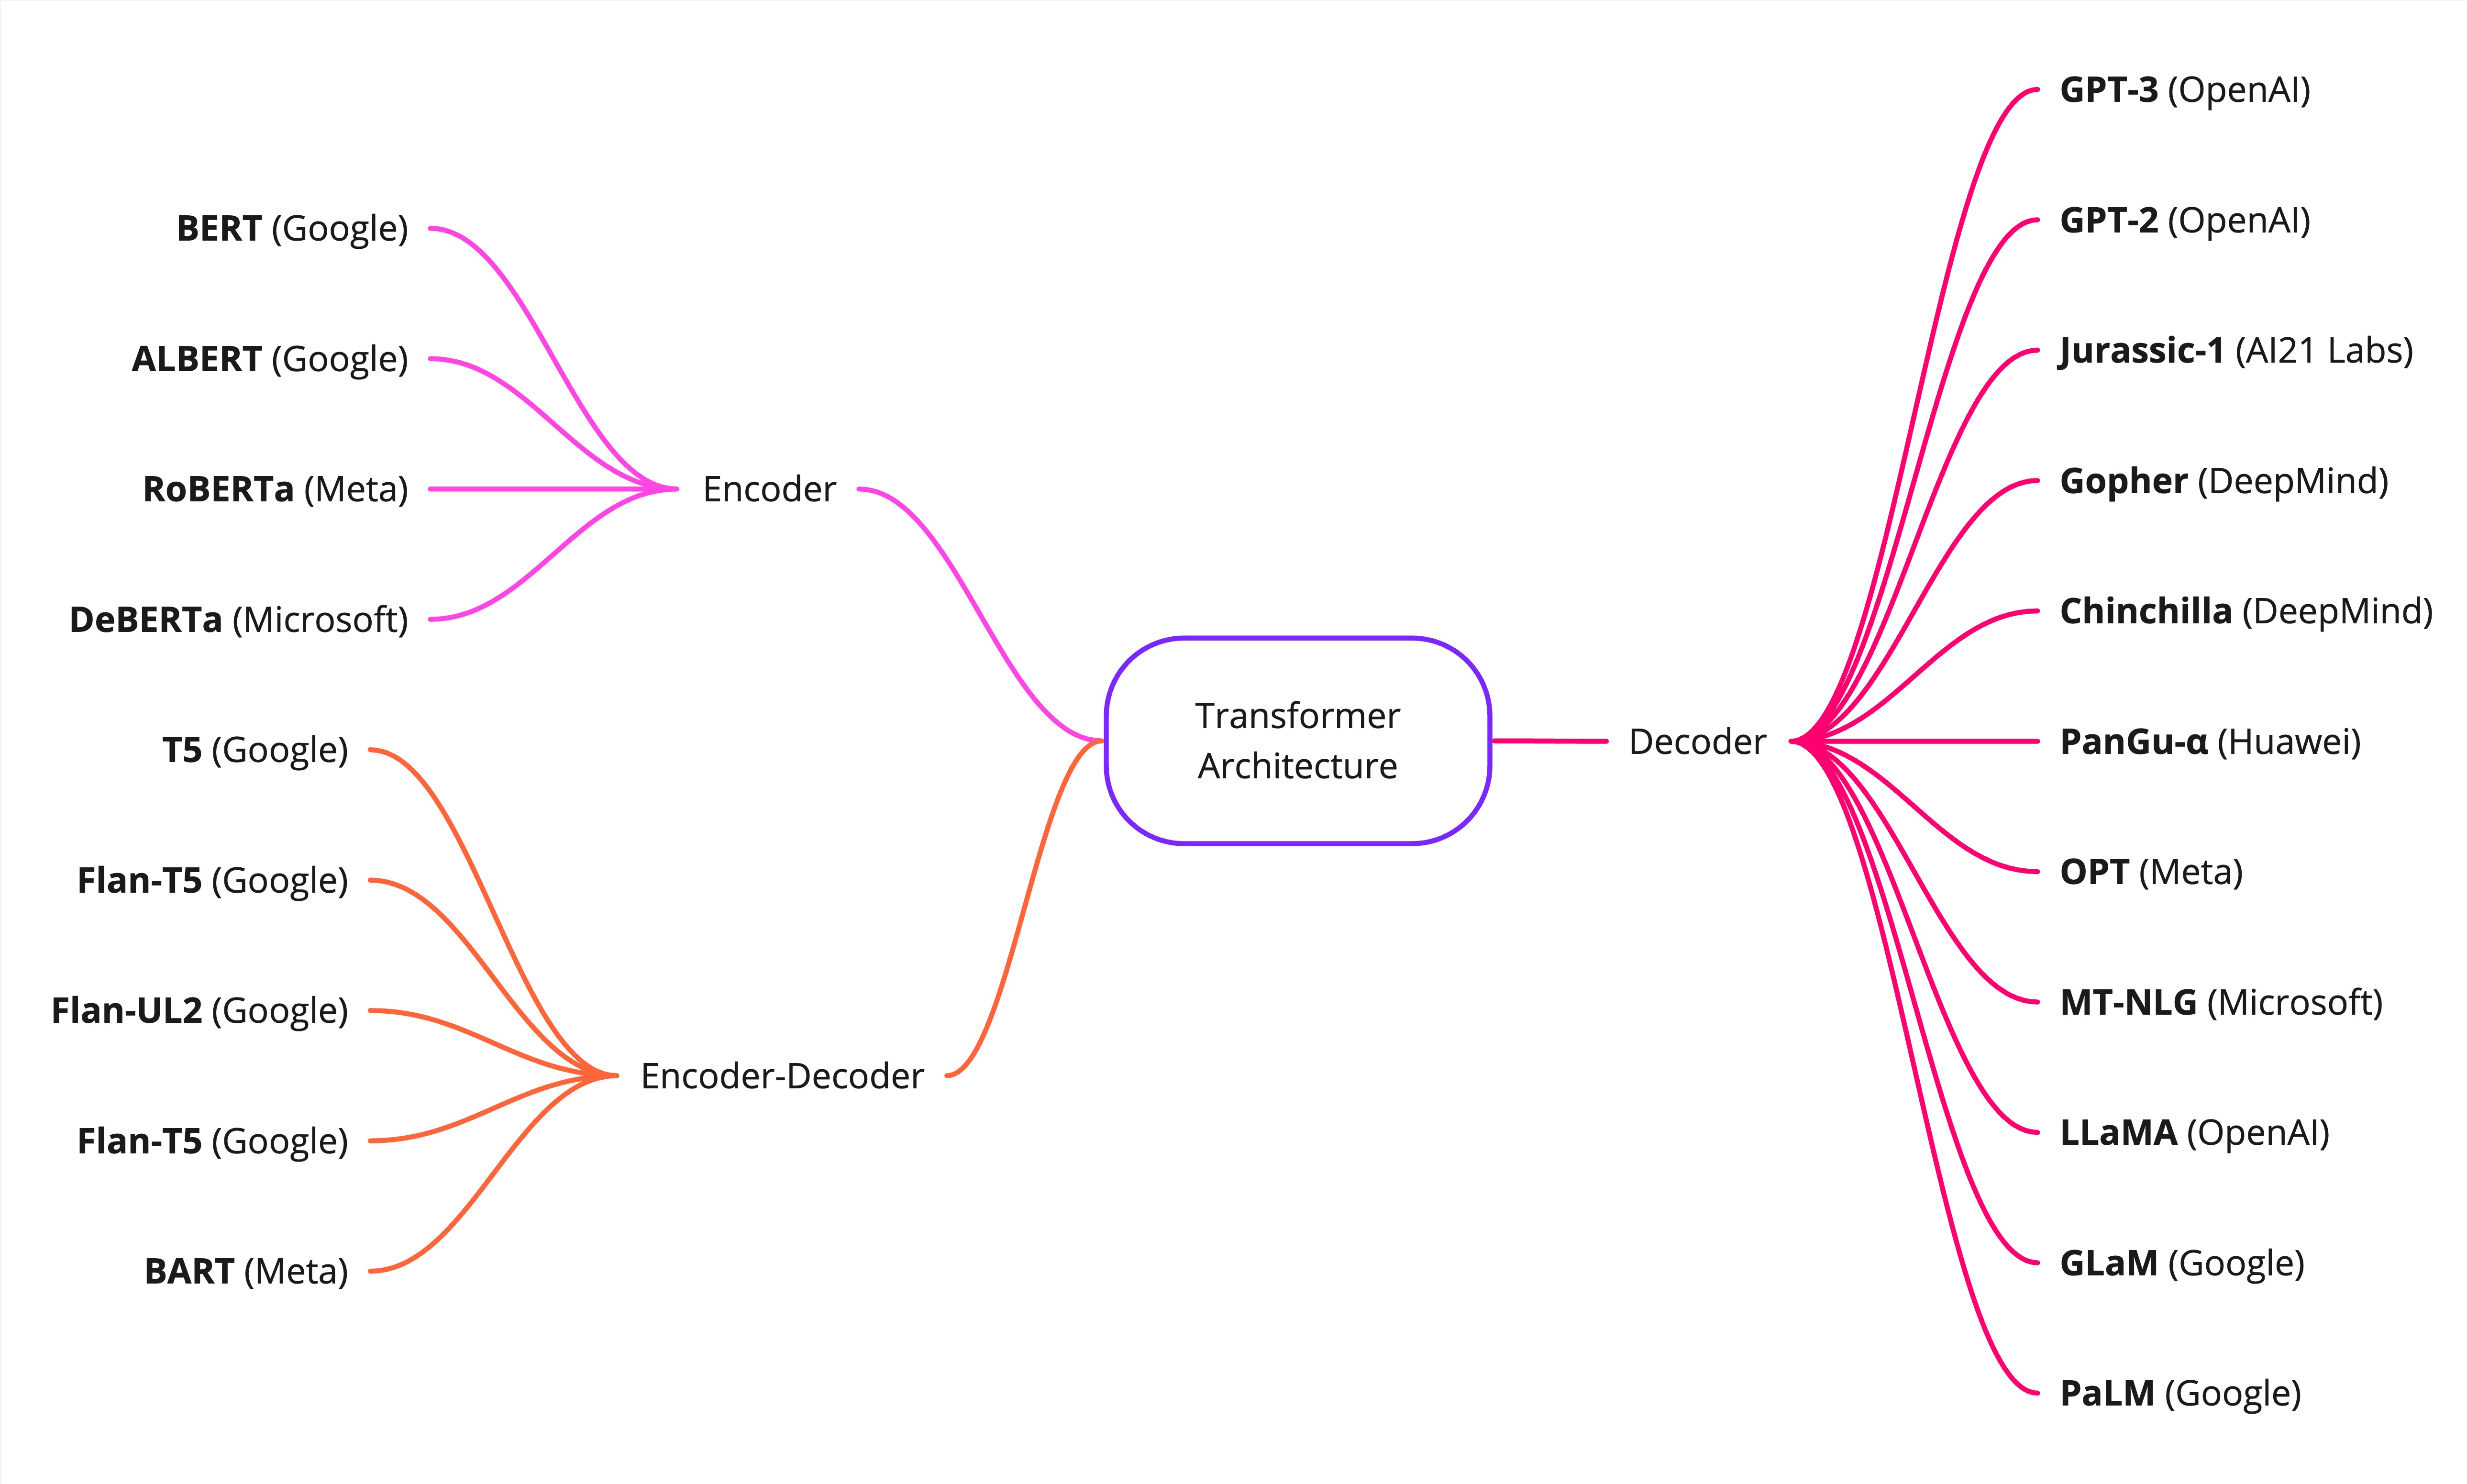
\includegraphics[width=\textwidth]{LLMs-Architectures}
	\caption{Some of the mainstream LLMs models by type.}
	\label{fig:llms-architectures}
\end{figure}

Mainstream architectures can be further categorized into three major types, namely encoder-decoder, casual decoder and prefix decoder as shown in Figure~\ref{fig:architectures}.
Both casual decoder and prefix decoder are decoder-only architectures, but they differ in the way they generate tokens.

\subsection{Encoder-decoder}
\label{subsec:encoder-decoder}

Vanilla version of the Transformer architecture introduced by \textcite{vaswani2023attention} belongs to this category, which consists of an encoder and a decoder.

The encoder's purpose is to transform an input sequence into a set of representations which capture its semantic and syntactic properties.

The decoder, on the other hand, is tasked with generating an output sequence from the encoded representations.
It predicts each token by conditioning on the previously generated tokens and the encoded input, a process that has seen significant improvements with the integration of cross-attention modules.
By segregating the understanding (encoding) and generation (decoding) processes, the Encoder-Decoder architecture enables a flexible approach to diverse language tasks.

So far, there are only a small number of models that use the encoder-decoder architecture (Figure~\ref{fig:llms-architectures}), such as BART~\cite{lewis2020bart} and T5~\cite{raffel2023exploring}.

\begin{figure}[h]
	\centering
	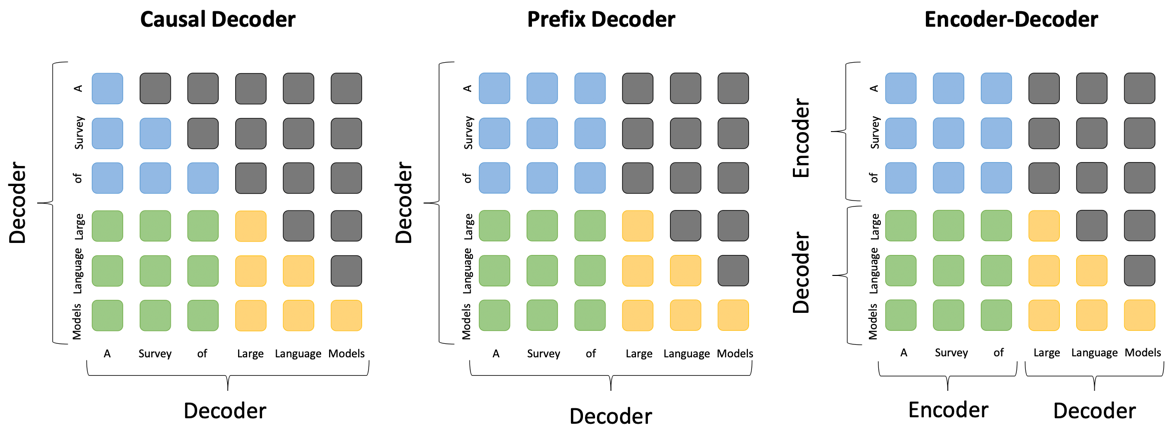
\includegraphics[width=\textwidth]{main_architectures}
	\caption{A comparison of the attention patterns in three mainstream architectures. Here, the blue, green, yellow and grey rounded rectangles indicate the attention between prefix tokens, attention between prefix and target tokens, attention between target tokens, and masked attention respectively. Source: \textcite{survey}.}
	\label{fig:architectures}
\end{figure}

\subsection{Casual decoder}
\label{subsec:casual-decoder}

In a causal decoder, each token is predicted based on the tokens that precede it, ensuring that the generation process is unidirectional and prevents the model from using future tokens in the prediction process~\cite{vaswani2023attention}.
This mechanism is akin to how humans produce language, one word at a time, building upon what has already been said without access to future words.

The architecture typically employs self-attention mechanisms where the attention distribution is masked to prevent tokens from attending to subsequent positions in the sequence (i.e., unidirectional attention mask).
This form of masking is instrumental in preserving the autoregressive property within the transformer-based models~\cite{radford2019language}.

The GPT series\footnote{GPT-3~\cite{brown2020language} showed amazing in-context learning capability, whereas GPT-1~\cite{radford2018improving} and GPT-2~\cite{radford2019language} didn't. It seems that scaling plays an important role in increasing the model capacity of this model architecture} of language models by OpenAI are prominent examples that utilize causal decoder architectures, where the ability to generate coherent and contextually relevant text has been demonstrated effectively~\cite{brown2020language}.

The causal decoder architecture is particularly well-suited for tasks that require sequential generation, such as text completion, language modeling, and text generation.
It has been widely adopted as the architecture of choice for many large-scale language models, such as OPT~\cite{zhang2022opt}, BLOOM~\cite{workshop2023bloom}, and Gopher~\cite{rae2021scaling}.

\subsection{Prefix decoder}
\label{subsec:prefix-decoder}

The prefix decoder architecture\footnote{Also called non-causal decoder~\cite{zhang2022examining}} enables partial conditioning of generated sequences, revising the masking mechanism of causal decoders, to enable performing bidirectional attention over the prefix tokens~\cite{dong2019unified} and unidirectional attention only on generated tokens.

In other words, this architecture allows the model to generate tokens based on both the input prefix and the target prefix, which can be useful for tasks that require generating sequences with specific prefixes or constraints.
In practice, a prefix decoder is implemented by feeding a fixed sequence of tokens \footnote{Also known as the prefix} into the decoder alongside the tokens generated so far.
The model then extends the prefix by generating subsequent tokens that logically follow the context provided by the prefix.

Unlike the causal decoder, which strictly adheres to a unidirectional generation pattern, the prefix decoder allows for a predefined context or prefix to guide the generative process~\cite{li2021prefixtuning}.
This is particularly useful in tasks such as machine translation, where the prefix can be a part of the translation that is already known or hypothesized, but the flexibility provided by the prefix decoder makes it suitable for a range of applications, from controlled text generation to task-oriented dialog systems, where maintaining context and coherence is crucial~\cite{li2022ptuning}.

This architecture has been utilized in various language models to improve control over text generation and to enhance the models' ability to handle specific formats or styles~\cite{raffel2023exploring}.

\subsection{Transformer Architecture}
\label{subsec:transformer-architecture}

The Transformer architecture has emerged as the de facto standard for LLMs, owing to its ability to capture long-range dependencies and model complex language structures effectively~\cite{vaswani2023attention} making possible to train models with billions or even trillions of parameters~\cite{brown2020language, touvron2023llama}.

This architecture usually consists of stacked Transformer layers (Figure~\ref{fig:architecture}), each comprising multi-head self-attention sub-layer and a position-wise fully connected feed-forward network~\cite{vaswani2023attention}.
Residual connection~\cite{he2016deep} and layer normalization~\cite{ba2016layer} are applied for both sub-layers individually.

\begin{figure}[H]
	\centering
	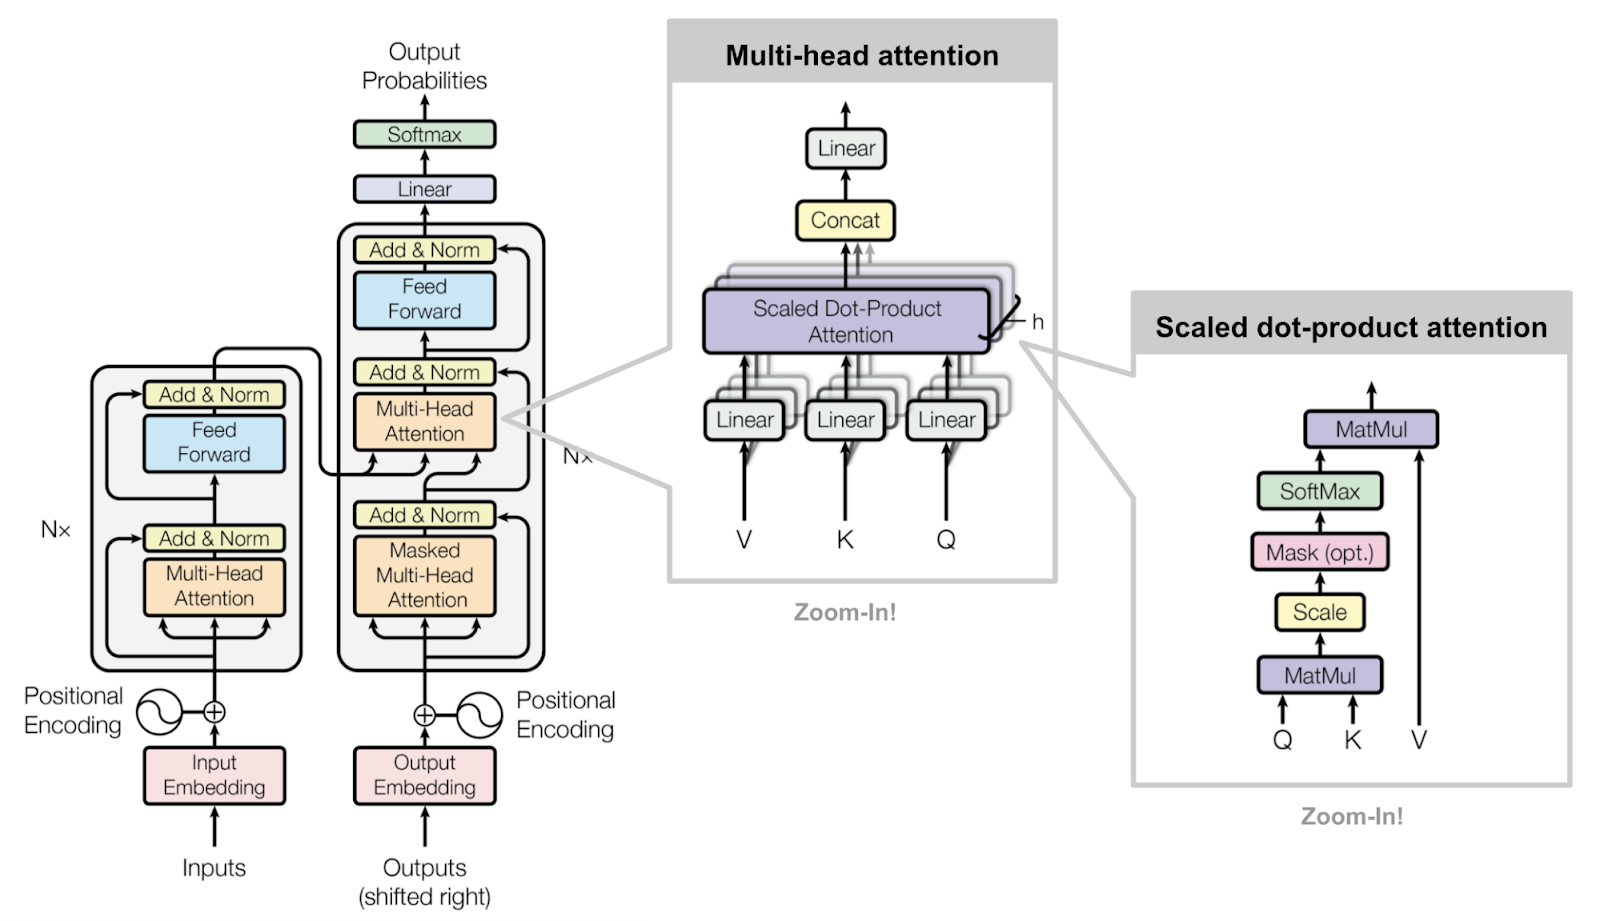
\includegraphics[width=\textwidth]{transformer_architecture}
	\caption{The full model architecture of the transformer. Source: \textcite{weng2018attention}.}
	\label{fig:architecture}
\end{figure}

The position-wise FFN sub-layer is a two-layer feed-forward network with a ReLU activation function between the layers.
Given a sequence of vectors \(h_1, h_2, \ldots, h_n\), the computation of a position-wise FFN sub-layer on any \(h_i\), as shown in Equation~\ref{eq:ffn}.

\begin{equation}
	\text{FFN}(h_i) = \text{ReLU}(h_{i}W^1 + b^1)W^2 + b^2
	\label{eq:ffn}
\end{equation}

\noindent where \(W^1\), \(W^2\), \(b^1\), and \(b^2\) are learnable parameters of the FFN sub-layer.

Besides the two sub-layers described above, the residual connection and layer normalization are also key components to the
Transformer.
Different orders and configuration of the sub-layers, residual connection and layer normalization in a Transformer layer lead to variants of Transformer architectures as shown in Table~\ref{tab:model-cards}.

\begin{table}[htb]
	\centering
	\scriptsize
	\begin{tabularx}{\textwidth}{|l|X|l|l|l|l|l|l|l|l|l|}
		\hline
		Model                                  & Category               & Size & Normalization & PE       & Activation & Bias & \#L & \#H & d\textsubscript{model} & MCL  \\
		\hline
		GPT3~\cite{brown2020language}          & Causal\newline decoder & 175B & Pre LayerNorm & Learned  & GeLU       & Y    & 96  & 96  & 12288                  & 2048 \\
		PanGU-\(\alpha\)~\cite{zeng2021pangu}  & Causal\newline decoder & 207B & Pre LayerNorm & Learned  & GeLU       & Y    & 64  & 128 & 16384                  & 1024 \\
		OPT~\cite{zhang2022opt}                & Causal\newline decoder & 175B & Pre LayerNorm & Learned  & ReLU       & Y    & 96  & 96  & 12288                  & 2048 \\
		PaLM~\cite{chowdhery2022palm}          & Causal\newline decoder & 540B & Pre LayerNorm & RoPE     & SwiGLU     & N    & 118 & 48  & 18432                  & 2048 \\
		BLOOM~\cite{workshop2023bloom}         & Causal\newline decoder & 176B & Pre LayerNorm & ALiBi    & GeLU       & Y    & 70  & 112 & 14336                  & 2048 \\
		MT-NLG~\cite{smith2022deepspeed}       & Causal\newline decoder & 530B & -             & -        & -          & -    & 105 & 128 & 20480                  & 2048 \\
		Gopher~\cite{rae2021scaling}           & Causal\newline decoder & 280B & Pre RMSNorm   & Relative & -          & -    & 80  & 128 & 16384                  & 2048 \\
		Chinchilla~\cite{hoffmann2022training} & Causal\newline decoder & 70B  & Pre RMSNorm   & Relative & -          & -    & 80  & 64  & 8192                   & -    \\
		Galactica~\cite{taylor2022galactica}   & Causal\newline decoder & 120B & Pre LayerNorm & Learned  & GeLU       & N    & 96  & 80  & 10240                  & 2048 \\
		LaMDA~\cite{thoppilan2022lamda}        & Causal\newline decoder & 137B & -             & Relative & GeGLU      & -    & 64  & 128 & 8192                   & -    \\
		Jurassic-1~\cite{lieber2021jurassic}   & Causal\newline decoder & 178B & Pre LayerNorm & Learned  & GeLU       & Y    & 76  & 96  & 13824                  & 2048 \\
		LLaMA~\cite{touvron2023llama}          & Causal\newline decoder & 65B  & Pre RMSNorm   & RoPE     & SwiGLU     & Y    & 80  & 64  & 8192                   & 2048 \\
		LLaMA 2~\cite{touvron2023llama2}       & Causal\newline decoder & 70B  & Pre RMSNorm   & RoPE     & SwiGLU     & Y    & 80  & 64  & 8192                   & 4096 \\
		Falcon~\cite{penedo2023refinedweb}     & Causal\newline decoder & 40B  & Pre LayerNorm & RoPE     & GeLU       & N    & 60  & 64  & 8192                   & 2048 \\
		GLM-130B~\cite{zeng2022glm130b}        & Prefix\newline decoder & 130B & Post DeepNorm & RoPE     & GeGLU      & Y    & 64  & 96  & 12288                  & 2048 \\
		T5~\cite{raffel2023exploring}          & Encoder-decoder        & 11B  & Pre RMSNorm   & Relative & ReLU       & N    & 24  & 128 & 1024                   & 512  \\
		\hline
	\end{tabularx}
	\caption{Model cards of several selected LLMs with public configuration details. PE denotes position embedding, \#L denotes the number of layers, \#H denotes the number of attention heads, d\textsubscript{model} denotes the size of hidden states, and MCL denotes the maximum context length during training. Source: \textcite{survey}.}
	\label{tab:model-cards}
\end{table}

\subsubsection{Configurations}
\label{subsubsec:configurations}

Since the introduction of the Transformer architecture, several variants and configurations have been proposed to improve the performance and efficiency of LLMs.
The configuration of the four major parts of the Transformer architecture includes normalization, position embeddings, activation functions, and attention and bias as shown in Table~\ref{tab:configurations}.

\subsubsection{Normalization Methods}
\label{subsubsec:normalization}
Normalization methods are crucial for stabilizing the training process and improving the convergence of LLMs.
In the vanilla Transformer~\cite{vaswani2023attention} architecture, LayerNorm~\cite{ba2016layer} is the most commonly used normalization method, which normalizes the hidden states across the feature dimension.
Before LayerNorm was introduced, BatchNorm~\cite{ioffe2015batch} was widely used in convolutional neural networks, but it was found to be less effective in sequence models due to the varying batch sizes and sequence lengths.
LayerNorm addresses this issue by normalizing the hidden states across the feature dimension, making it more suitable for sequence models.
Specifically, LayerNorm normalizes the hidden states using the mean and the variance of the summed inputs within each layer.

RMSNorm~\cite{zhang2019root} is another normalization method that has been proposed to improve the training speed of LayerNorm.
RMSNorm normalizes the hidden states by dividing them by the root mean square of the squared hidden states, which has been shown to improve the training speed and performance~\cite{narang2021transformer}.
ChinchiLLa~\cite{hoffmann2022training} amd Gopher~\cite{rae2021scaling} are examples of LLMs that use RMSNorm as the normalization method.

DeepNorm~\cite{wang2022deepnet} is a novel normalization method that combines LayerNorm with a learnable scaling factor to stabilize the training process of deep Transformer models.
With DeepNorm, Transformer models can be scaled up to hundreds of layers without the need for additional normalization layers, making it an effective method for training large-scale LLMs~\cite{wang2022deepnet}.
It has been used in models such as GLM-130B~\cite{zeng2022glm130b}.

\begin{table}[htbp]
	\begin{tabularx}{\textwidth}{|X|X|}
		\hline
		\textbf{Configuration} & \textbf{Method}                        \\
		\hline
		Normalization position & Post Norm~\cite{vaswani2023attention}  \\
		                       & Pre Norm~\cite{radford2019language}    \\
		                       & Sandwich Norm~\cite{ding2021cogview}   \\
		Normalization method   & LayerNorm~\cite{ba2016layer}           \\
		                       & RMSNorm~\cite{zhang2019root}           \\
		                       & DeepNorm~\cite{wang2022deepnet}        \\
		Activation function    & ReLU~\cite{nair2010rectified}          \\
		                       & GeLU~\cite{wang2018glue}               \\
		                       & Swish~\cite{ramachandran2017searching} \\
		                       & SwiGLU~\cite{shazeer2020glu}           \\
		                       & GeGLU~\cite{shazeer2020glu}            \\
		Position embedding     & Absolute~\cite{vaswani2023attention}   \\
		                       & Relative~\cite{raffel2023exploring}    \\
		                       & RoPE~\cite{su2021roformer}             \\
		                       & Alibi~\cite{press2022train}            \\
		\hline
	\end{tabularx}
	\caption{Detailed formulations for the network configurations. Source: \textcite{survey}}
	\label{tab:configurations}
\end{table}

\subsubsection{Normalization Position}
\label{subsubsec:normalization-position}

\begin{figure}
	\centering
	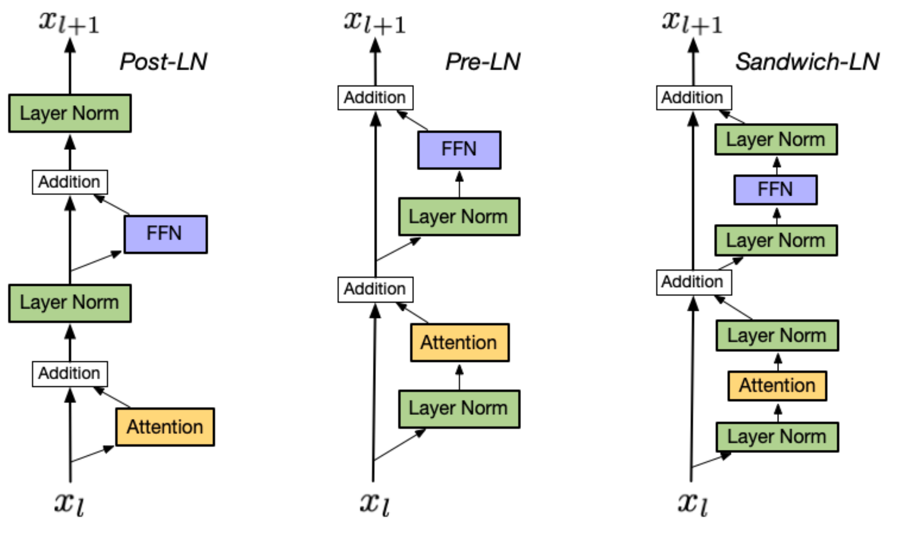
\includegraphics[width=\textwidth]{prepostln}
	\caption{Illustration of different LayerNorm structures in Transformers. Source: \textcite{ding2021cogview}.}
	\label{fig:prepostln}
\end{figure}

The position of the normalization layer (Figure~\ref{fig:prepostln}) in the Transformer architecture can have a significant impact on the model's performance and convergence.
The three main configurations proposed in different studies are pre-LN\footnote{Pre-Layer Normalization}, post-LN\footnote{Post-Layer Normalization}, and Sandwich-LN\@.

In the pre-LN configuration, the normalization layer is placed inside the residual blocks, while in the post-LN configuration, the normalization layer is placed after the residual blocks.
In \textcite{ding2021cogview}, the normalization layer is placed both before and after the residual blocks, which is referred to as the Sandwich-LN configuration.

Post-LN is used in the vanilla Transformer architecture~\cite{vaswani2023attention}, where the normalization layer is placed between the residual blocks.
This sequence allows the model to first process the input through a sublayer, such as a Multi-Head Attention (MHA) or Feed-Forward Network (FFN), and then apply normalization to the output of the sublayer combined with the residual connection.
In particular, to train the model from scratch, any gradient-based optimization approach requires a learning rate warm-up stage to stabilize the training process~\cite{vaswani2023attention}.
Existing works found that training of Transformer models with post-norm tends to be instable due to large gradients near the output layer~\cite{xiong2020layer}.

Pre-LN~\cite{baevski2019adaptive} is another configuration where the normalization layer is placed inside the residual blocks and makes possible to remove warm-up stage, requiring significantly less training time and hyper-parameter tuning on a wide range of applications.
The Transformers with pre-LN have shown to be more stable during training but have worst performance~\cite{liu2020understanding}.

Sandwich-LN~\cite{ding2021cogview} is a configuration that combines the advantages of both pre-LN and post-LN by placing the normalization layer both before and after the residual blocks.
This configuration has been shown to improve the performance of Transformer models by providing better stability during training and faster convergence~\cite{ding2021cogview}.
In \textcite{zeng2022glm130b}, the authors found that the Sandwich-LN configuration sometimes fails to stabilize the training of LLMs and may lead to the collapse of training.

\subsubsection{Activation Functions}
\label{subsubsec:activation-functions}

Activation functions play a crucial role in the training and performance of LLMs by introducing non-linearity into the model\footnote{In the feed-forward layer}.
The most commonly used activation functions in LLMs are ReLU, GeLU, Swish, SwiGLU, and GeGLU\@.

ReLU\footnote{Rectified Linear Unit}~\cite{nair2010rectified} is a simple and widely used activation function that introduces non-linearity by setting negative values to zero.

\begin{equation}
	\text{ReLU}(x) = \max(x, 0)
	\label{eq:relu}
\end{equation}

One of the first activation functions to be used in deep learning, ReLU has been shown to be effective in training deep neural networks by preventing the vanishing gradient problem~\cite{glorot2011deep}.
This non-linear activation function introduces sparsity in the activations of the network, which can lead to faster training and better performance due to its simplicity and efficiency.
However, ReLU can suffer from the dying ReLU problem, where neurons can become inactive and stop learning if the input is negative~\cite{maas2013rectifier}.

GeLU~\cite{hendrycks2016gaussian} is a Gaussian Error Linear Unit activation function that is used to model uncertainties in neural networks.
It was introduced to improve upon ReLU by taking into account the stochastic regularisation techniques.
The smoothness of the GELU function can be advantageous in deep neural networks with many layers, as it can help prevent the problem of "dying ReLU" and improve the flow of gradients through the network.
The GELU activation function is mathematically described as:

\begin{equation}
	\text{GeLU}(x) = x \cdot \Phi(x)
	\label{eq:geluf}
\end{equation}

\noindent where \(\Phi(x)\) is the cumulative distribution function of the standard Gaussian distribution.
This can also be approximated as:

\begin{equation}
	\text{GeLU}(x) \approx 0.5x(1 + \tanh[\sqrt{2/\pi}(x + 0.044715x^3))]
	\label{eq:geluapprox1}
\end{equation}

Alternatively, the GELU function can be expressed as a scaled version of the sigmoid function, as shown below:

\begin{equation}
	\text{GeLU}(x) \approx x \cdot \sigma(1.702x)
	\label{eq:geluapprox2}
\end{equation}

The GELU function allows the input to control its own gate, deciding whether to pass through or be dampened.
When x is large, GELU approximates to x, acting like a linear unit.
When x is close to zero or negative, it squashes the output, making it closer to zero.
In other words, the GELU function would produce outputs that are smoothed around zero, rather than sharply cut off as with ReLU\@.
The GELU activation function is used in many deep learning models, including GPT-3 and BERT\@.

The Swish~\cite{ramachandran2017searching} activation function is a smooth, non-monotonic function that was developed to overcome some limitations of ReLU and was found to perform better in deeper models.
It is defined as

\begin{equation}
	\text{Swish} = x \cdot \sigma\left(x\right)
	\label{eq:swish}
\end{equation}

\noindent where x is the input to the activation function and sigmoid is the logistic function \(\sigma(x) = \frac{1}{1+e^{-x}}\).
The Swish function allows small and negative values to pass through, which can be beneficial for gradient flow in deep models.
It has been empirically demonstrated to work well for deeper models and is computationally efficient.

SwiGLU~\cite{shazeer2020glu} is a variant of the Swish activation function that combines the Swish function with the Gated Linear Unit (GLU) function.
The SwiGLU activation function is defined as

\begin{equation}
	\text{SwiGLU}\left(x, W, V, b, c, \beta\right) = \text{Swish}\left(xW + b\right) \otimes \left(xV + c\right)
	\label{eq:swiglu}
\end{equation}

\noindent Here, x is the input to the neuron, W and V are weight matrices, b and c are bias vectors, and $\beta$ is a constant.
The $\otimes$ symbol denotes element-wise multiplication, while Swish is the activation function described in Equation~\ref{eq:swish}.
This function allows the network to learn which parts of the input should be retained (gated) for further layers, combining the advantages of non-saturating functions and dynamic gating mechanisms.

GeGLU~\cite{shazeer2020glu} is another variant of the GLU activation function that combines the GeLU function with the Gated Linear Unit (GLU) function.
The GeGLU activation is formulated as:

\begin{equation}
	\text{GeGLU}\left(x, W, V, b, c\right) = \text{GeLU}\left(xW + b\right) \otimes \left(xV + c\right)
	\label{eq:geglu}
\end{equation}

\noindent After the output of the GeLU function is calculated, it is multiplied element-wise with a second matrix.
This second matrix is calculated by multiplying the input matrix x with another matrix W and adding a bias term b.
The output of this multiplication is then passed through a second matrix V and added to a scalar term c.

\subsubsection{Position Embeddings}
\label{subsubsec:position-embeddings}

Position embeddings are a crucial component of the Transformer architecture that allows the model to capture the sequential order of tokens in the input sequence.
There are several types of position embeddings used in LLMs, including absolute, relative, RoPE, and Alibi embeddings.

Absolute position embeddings~\cite{vaswani2023attention} was proposed in the original Transformer model.
At the bottoms of the encoder and the decoder, the absolute positional embeddings are added to the input embeddings.
There are two variants of absolute position embeddings, i.e., sinusoidal and learned position embeddings, where the latter is commonly used in existing pre-trained language models.

The formulation for adding absolute position embeddings is straightforward:

\begin{equation}
	E_{\text{total}}(i) = E_{\text{token}}(i) + E_{\text{position}}(i)
	\label{eq:absolute-position-embeddings}
\end{equation}

\noindent where \(E_{\text{total}}(i)\) is the final embedding vector for token \(i\), \(E_{\text{token}}(i)\) is the initial token embedding for token \(i\), and \(E_{\text{position}}(i)\) is the position embedding vector for token \(i\).
This technique allows the model to use the order of words to understand meaning and context, which is especially important for tasks involving sequence modeling and generation.

Relative position embeddings~\cite{shaw2018self} are an alternative to absolute position embeddings that capture the relative distance between tokens in the input sequence.
This allows the model to learn more flexible and adaptive representations of the input sequence, which can improve performance on tasks that require capturing long-range dependencies and complex relationships between tokens.
Relative position embeddings are incorporated into the self-attention mechanism of Transformer models.
Instead of only considering the absolute position of tokens, the attention scores are adjusted based on the relative distances between tokens.
The formulation for the attention mechanism with relative position embeddings is given by:

\begin{equation}
	\text{Attention}(Q, K, V) = \text{softmax}\left(\frac{Q(K+R)^T}{\sqrt{d_k}}\right)V
	\label{eq:relative-position-embeddings}
\end{equation}

\noindent where \(Q\), \(K\), and \(V\) are the query, key, and value matrices, respectively, \(R\) is the relative position embedding matrix, and \(d_k\) is the dimension of the key vectors.
The relative positions are calculated as \(R_{ij} = R_{pos[i]-pos[j]}\), where \(pos[i]\) and \(pos[j]\) are the positions of tokens \(i\) and \(j\) in the input sequence, respectively.

RoPE\footnote{Rotary Position Embeddings}~\cite{su2021roformer} is a type of position embedding that uses rotational matrices to capture the relative positions of tokens in the input sequence.
Unlike traditional position embeddings that add or concatenate position information, RoPE encodes position information through rotation in the embedding space, enabling models to preserve positional relationships effectively.
The key idea of RoPE is to bind the position encoding with the word embedding in a way that preserves the rotational relationship between embeddings.
It uses a rotation matrix to modulate the embedding based on its position, thereby aligning words by their relative positions instead of their absolute positions.
The formula for the Rotary Position Embedding is:

\begin{equation}
	E_{\text{rot}}(x_i,p_i) = \text{Rotate}(x_i,p_i) = x_i\cos(p_i) + (Wx_i)\sin(p_i)
	\label{eq:rope}
\end{equation}

\noindent where \(x_i\) is the token embedding, \(p_i\) is the position embedding, and \(W\) is a learnable weight matrix.
Rotary Position Embeddings were introduced by \textcite{su2021roformer} and have been shown to improve the performance of LLMs on a range of tasks.

ALiBi\footnote{Attention with Linear Biases}~\cite{press2022train} position embeddings offer an alternative mechanism for incorporating position information into Transformer models.
Unlike traditional absolute or relative position embeddings, ALiBi introduces biases directly into the self-attention mechanism to handle positional dependencies.
ALiBi introduces a linear bias based on the distance between tokens in the attention scores.
Similar to relative position embedding, it biases attention scores with a penalty based on the distances between keys and queries.
Different from the relative positional embedding methods like T5~\cite{zeng2021pangu}, the penalty scores in ALiBi are pre-defined without any trainable parameters.
This bias is subtracted from the attention logits before the softmax operation, helping the model to prioritize nearby tokens over distant ones, which is crucial in many sequential tasks.
The modified attention score with ALiBi can be represented as:

\begin{equation}
	\begin{aligned}
		\text{Attention}(Q, K, V) & = \text{softmax}\left(\frac{QK^T}{\sqrt{d_k}} - \text{bias}(i,j)\right)V, \\
		\text{bias}(i,j)          & = b \cdotp |i-j|
	\end{aligned}
	\label{eq:alibi}
\end{equation}

\noindent where \(Q\), \(K\), and \(V\) are the query, key, and value matrices, respectively, and \(b\) is a learnable scalar parameter that controls the strength of the bias, and \(|i-j|\) is the absolute distance between tokens \(i\) and \(j\), and \(d_k\) is the dimension of the key vectors.

In \textcite{press2022train}, the authors found that ALiBi has better extrapolation performance than traditional position embeddings, and it can also improve the stability and convergence of Transformer models during training~\cite{workshop2023bloom}.

\subsubsection{Attention Mechanisms}
\label{subsubsec:attention-mechanisms}

Attention mechanisms are a key component of the Transformer architecture that allows the model to capture long-range dependencies and complex relationships between tokens in the input sequence.

An attention function can be described as mapping a query and a set of key-value pairs to an output, where the query, keys, values, and output are all vectors.
The output is computed as a weighted sum of the values, where the weight assigned to each value is computed by a compatibility function of the query with the corresponding key.
The two most commonly used attention functions are additive attention~\cite{bahdanau2014neural}, and dot-product (multiplicative) attention.
\begin{figure}[h]
	\centering
	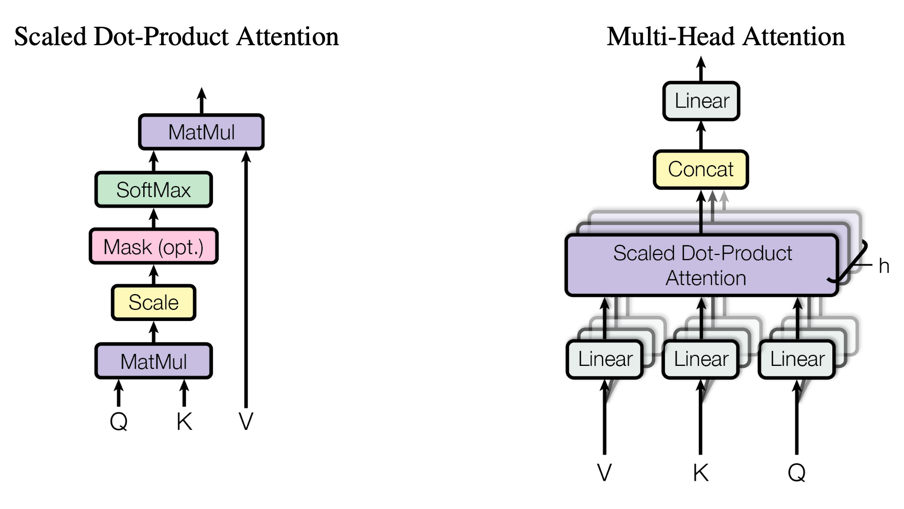
\includegraphics[width=0.8\textwidth]{attention}
	\caption{(left) Scaled Dot-Product Attention. (right) Multi-Head Attention consists of several attention layers running in parallel. Source: \textcite{vaswani2023attention}.}
	\label{fig:attention}
\end{figure}
The scaled dot-product attention function used in \textcite{vaswani2023attention} is defined as follows:

\begin{equation}
	\text{Attention}(Q, K, V) = \text{softmax}\left(\frac{QK^T}{\sqrt{d_k}}\right)V
	\label{eq:dot-scaled-attention}
\end{equation}

\noindent where \(Q\), \(K\), and \(V\) are the query, key, and value matrices, respectively, and d\textsubscript{k} is the dimension of the key vectors.
While for small values of d\textsubscript{k} the two mechanisms perform similarly, additive attention outperforms dot product attention without scaling for larger values of d\textsubscript{k}~\cite{britz2017massive}.

A multi-head attention functions is implemented by splitting the query, key, and value vectors into multiple heads and computing the attention function in parallel, yielding d\textsubscript{v}-dimensional output values.
These are concatenated and once again projected, resulting in the final values, as depicted in Figure~\ref{fig:attention}.
The multi-head attention mechanism allows the model to jointly attend to information from different representation subspaces at different positions, enhancing the model's capacity to capture complex relationships in the data.

\begin{equation}
	\begin{aligned}
		\text{MultiHead}(Q, K, V) & = \text{Concat}(\text{head}_1, \ldots, \text{head}_h)W^O, \\
		\text{head}_i             & = \text{Attention}(QW_i^Q, KW_i^K, VW_i^V)
	\end{aligned}
	\label{eq:multihead-attention}
\end{equation}

\noindent where \(W_i^Q\), \(W_i^K\), and \(W_i^V\) are the weight matrices for the query, key, and value projections of the \(i\)-th head, respectively, and \(W^O\) is the final output projection matrix.

We can categorize the attention mechanisms into: full attention, sparse attention, multi-query/grouped-query attention, Flash attention, and Paged attention.
The Full attention mechanism is the standard attention mechanism used in the vanilla Transformer architecture~\cite{vaswani2023attention}, where each token attends to all other tokens in the sequence.
It adopts the scaled dot-product we already discussed in Equation~\ref{eq:dot-scaled-attention}.
This mechanism is computationally expensive and has a quadratic complexity in terms of the number of tokens, which can limit the model's scalability to longer sequences.
To address this issue, several studies have proposed alternative attention mechanisms.

In the Sparse attention mechanism, tokens only attend to a subset of other tokens, according to a predefined pattern (e.g., local windows).
This mechanism reduces the computational complexity of the attention operation and allows the model to scale to longer sequences.

\begin{equation}
	\text{Sparse Attention}(Q, K, V) = \text{softmax}((\frac{QK^T \cdotp M}{\sqrt{d_k}}))V
	\label{eq:sparse-attention}
\end{equation}

\noindent where \(M\) is a sparse attention mask that defines the pattern of attention between tokens.

Various sparse attention mechanisms have been proposed in the literature, such as \textcite{peng2021random}, \textcite{zaheer2020big} and \textcite{child2019generating}.
It a useful in tasks involving very long documents or sequences, such as document classification and genomic sequence analysis.

The multi-query/grouped-query attention mechanism~\cite{shazeer2019fast} is an extension of the standard attention mechanism, where the keys and values are shared across all of the different attention "heads", greatly reducing the size of these tensors and hence the memory bandwidth requirements of incremental decoding.
This mechanism is particularly useful in tasks that require processing large amounts of data, such as machine translation and summarization.
It can significantly reduce the computational cost of the attention operation with small sacrifices in model quality.
Palm~\cite{chowdhery2022palm} and Starcoder~\cite{li2023starcoder} are examples of LLMs that use the multi-query attention mechanism.
A tradeoff between multi-query and multi-head attention, grouped-query (GQA) has been explored in \textcite{ainslie2023gqa}.
In GQA heads are grouped together, and each group attends share the same transformation matrices.
This mechanism has been adopted and empirically tested in LLaMA 2 model~\cite{touvron2023llama2}.

Flash attention~\cite{dao2022flashattention} is an approach that propose to optimize the speed and and memory consumption of attention module on the GPUs.
Modern GPUs have different memory types, and Flash attention takes advantage of this by organizing the input block on the faster memory\footnote{SRAM has fast IO, while HBM is slower}.
Updated version FlashAttention-2~\cite{liu2022fast} has been proposed to further improve the performance of the attention module on GPUs, partitioning of GPU thread blocks and warps, leading to around 2× speedup when compared to the original FlashAttention.

PagedAttention~\cite{vllm2023} is based on the observation that GPU memory is bottlenecked by cached attention keys and value tensors.
These cached key and value tensors are often referred to as KV cache.
The KV cache is large and highly dynamic, depending on the sequence length.
Authors finds that existent system waste 60\%-80\% of the memory due to fragmentation and over-reservation.
PagedAttention proposed techniques inspired by virtual memory management\footnote{Paging} to manage the KV cache, partition sequences to sub-sequences allocating corresponding KV caches into non-contiguous physical blocks as shown in Figure~\ref{fig:paging}.

\begin{figure}[h]
	\centering
	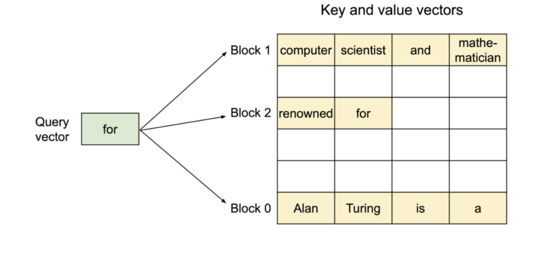
\includegraphics[width=0.8\textwidth]{pagedattentionblocks}
	\caption{PagedAttention: KV Cache are partitioned into blocks. Source: \textcite{vllm2023}.}
	\label{fig:paging}
\end{figure}

Paging increases the GPU memory utilization and enables efficient memory sharing in parallel sampling (Figure~\ref{fig:paging-parallel}).

\begin{figure}[h]
	\centering
	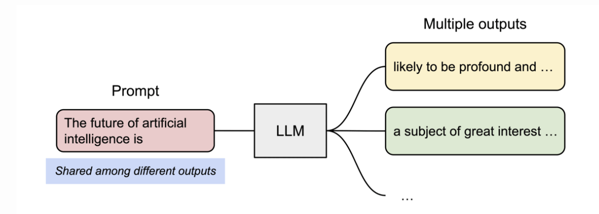
\includegraphics[width=0.8\textwidth]{pagedattentionparalle}
	\caption{PagedAttention: example of parallel sampling. Source: \textcite{vllm2023}.}
	\label{fig:paging-parallel}
\end{figure}

To put all these discussions together, \textcite{survey} summarize the suggestions from existing literature for detailed configuration.
For stronger generalization and training stability, it is suggested to choose the pre RMSNorm for layer normalization, and SwiGLU or GeGLU as the activation function.
In addition, LN may not be used immediately after embedding layers, which is likely to incur performance degradation.
As for position embeddings, RoPE or ALiBi is a better choice since it performs better on long sequences.

\subsection{Emerging architectures}
\label{subsec:emerging-architectures}

There are several emerging architectures that have been proposed to address specific challenges or improve the performance of the Transformers.
One of the main issues with the vanilla Transformer architecture is the quadratic complexity in terms of the number of tokens, which can limit the model's scalability to longer sequences.
To address this performance issue, several studies proposed alternative architectures, such as parameterized state space models (e.g., S4~\cite{gu2022efficiently}, GSS~\cite{mehta2022long}, and H3~\cite{dao2022hungry}]), long convolutions(e.g.,Hyena~\cite{poli2023hyena}), and recursive update mechanisms (RWKV~\cite{peng2023rwkv} and RetNet~\cite{sun2023retentive}).

Parameterized state space models are a class of models that use a parameterized state space to represent the hidden states of the model.
However, this method has prohibitive computation and memory requirements, rendering it infeasible as a general sequence modeling solution.
To address this issue, S4~\cite{gu2022efficiently} proposed a novel parameterized state space model that uses a fixed-size state space to represent the hidden states of the model.
This approach significantly reduces the computational and memory requirements of the model while maintaining high performance on a range of tasks.
In \textcite{gu2022efficiently}, the authors found that S4 can be trained quickly and efficiently efficient compared to Transformer variants designed for long-range sequence modeling as shown in Table~\ref{tab:ssm_efficiency}.

\begin{table}[htbp]
	\centering
	\begin{tabularx}{0.6\textwidth}{Xcccc}
		\toprule
		            & \multicolumn{2}{c}{LENGTH 1024} & \multicolumn{2}{c}{LENGTH 4096}                                    \\
		\cmidrule(lr){2-3} \cmidrule(lr){4-5}
		            & Speed                           & Mem.                            & Speed          & Mem.            \\
		\midrule
		Transformer & 1x                              & 1x                              & 1x             & 1x              \\
		S4          & \textbf{1.58x}                  & \textbf{0.43x}                  & \textbf{5.19x} & \textbf{0.091x} \\
		\bottomrule
	\end{tabularx}
	\caption{Benchmarks vs. efficient Transformers}
	\label{tab:ssm_efficiency}
\end{table}

Long Range Arena(LRA)~\cite{tay2021longrange} is a benchmark suite that evaluates the performance of LLMs on a range of tasks that require capturing long-range dependencies.
It contains 6 tasks with lengths 1K-16K steps, encompassing modalities and objectives that require similarity, structural, and visuospatial reasoning.
Table~\ref{tab:LRA} shows the performance of S4 and 11 Transformer variants from \textcite{tay2021longrange}.
Notably, S4 solves the Path-X task, an extremely challenging task that involves reasoning about LRDs over sequences of length 128 × 128 = 16384.
All previous models have failed (i.e., random guessing) due to memory or computation bottlenecks, or simply being unable to learn such long dependencies.
\begin{table}[htbp]
	\centering
	\begin{tabularx}{\textwidth}{Xccccccccc}
		\toprule
		MODEL       & ListOps        & Text           & Retrieval      & Image          & Pathfinder     & Path-X         & AVG            \\
		\midrule
		Transformer & 36.37          & 64.27          & 57.46          & 42.44          & 71.40          & X              & 53.66          \\
		\addlinespace
		S4          & \textbf{58.35} & \textbf{76.02} & \textbf{87.09} & \textbf{87.26} & \textbf{86.05} & \textbf{88.10} & \textbf{80.48} \\
		\bottomrule
	\end{tabularx}
	\caption{(Long Range Arena) Accuracy on full suite of LRA tasks. (Top) Original Transformer variants in LRA. Source: \textcite{gu2022efficiently}.}
	\label{tab:LRA}
\end{table}
Other benchmarks in \textcite{gu2022efficiently} show that S4 looks promising for long-range sequence modeling, achieving state-of-the-art performance on a range of tasks that require capturing long-range dependencies.

Long convolutions are a class of models that use convolutional layers to capture long-range dependencies in the input sequence. \textcite{poli2023hyena} proposed an operation-efficient architecture called Hyena defined by two recurring sub-quadratic operators: a long convolution and an element-wise multiplicative gating (Figure~\ref{fig:hyena}).
Compared to attention operator in Transformers, Hyena has a lower computational complexity and memory footprint, making it more efficient for long-range sequence modeling.

\begin{figure}[h]
	\centering
	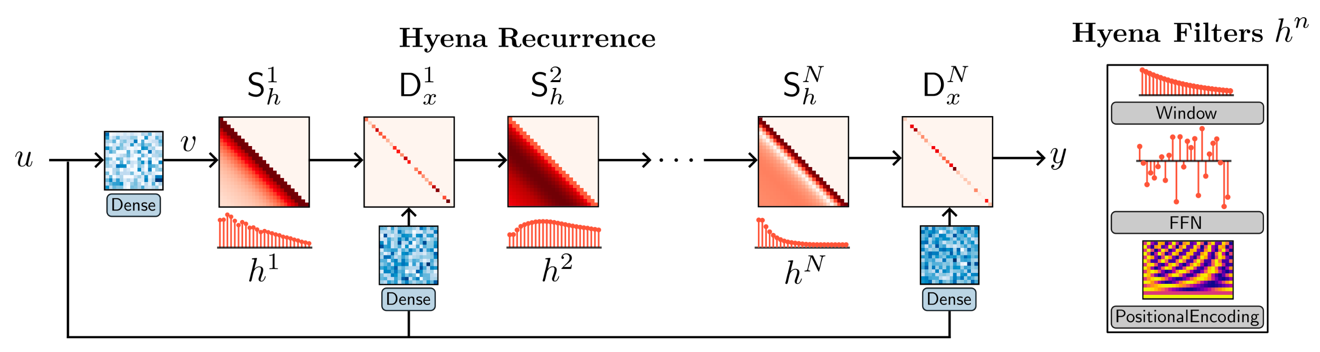
\includegraphics[width=0.8\textwidth]{hyena}
	\caption{The Hyena operator is defined as a recurrence of two efficient subquadratic primitives: an implicit long convolution h (i.e., Hyena filters parameterized by a feed-forward network) and multiplicative element-wise gating of the (projected) input. The depth of the recurrence specifies the size of the operator. Source: \textcite{poli2023hyena}.}
	\label{fig:hyena}
\end{figure}

\section{Tuning and Optimization}
\label{sec:tuning-optimization}

Since LLMs consist of millions or billions of parameters, parameter tuning can be expensive and time-consuming.
In this section, we discuss model adaptation of parameters and memory.

\subsection{Parameter-efficient model adaptation}
\label{subsec:parameter-efficient}

In the existent literature, there are several methods to adapt the model parameters to improve the performance of LLMs~\cite{hu2021lora, li2021prefixtuning, lester2021power}.
The goal of these methods is to reduce the number of parameters in the model while maintaining performance as much as possible.
In the following sections, we discuss some of the most popular methods for parameter-efficient model adaptation, such as adapter tuning, prefix tuning, prompt tuning, and and LoRA (illustrated in Figure~\ref{fig:parameter-tuning}).

\begin{figure}[h]
	\centering
	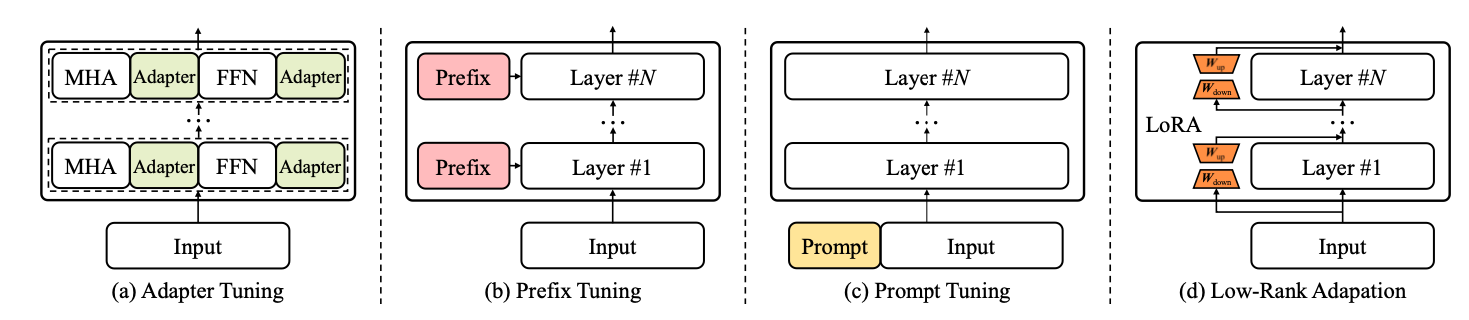
\includegraphics[width=\textwidth]{parameter-tuning}
	\caption{An illustration of four different parameter-efficient fine-tuning methods. MHA and FFN denote the multi-head
		attention and feed-forward networks in the Transformer layer, respectively. Source: \textcite{survey}.}
	\label{fig:parameter-tuning}
\end{figure}

\subsubsection{Adapter tuning}
\label{subsubsec:adapter-tuning}

Adapter tuning is a parameter-efficient technique for transferring a pre-trained model to multiple downstream tasks without re-training the entire model for each new task.
This approach involves introducing small, trainable modules called "adapters" between the layers of a pre-trained network, allowing the original network's parameters to remain fixed while adapting the model to new tasks with a minimal increase in the total number of parameters.
Adapter tuning is designed to address the inefficiency of fine-tuning large models where each new task typically requires re-training the entire model.
Instead, adapter tuning uses a base pre-trained model and introduces small adapter layers that are trained for each specific task into the Transformer architecture~\cite{houlsby2019parameterefficient, hu2023llmadapters}, as shown in Figure~\ref{fig:adapter-architecture}.

\begin{figure}[h]
	\centering
	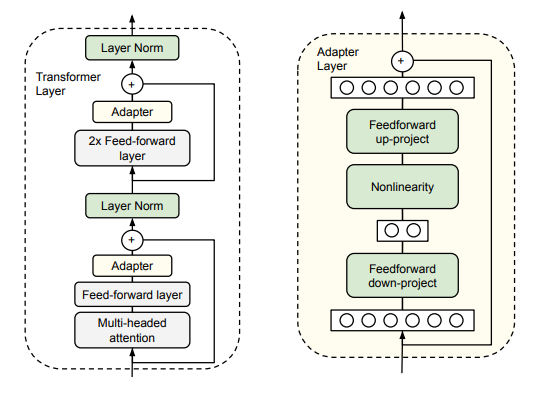
\includegraphics[width=0.8\textwidth]{adapter-architecture}
	\caption{On the left, the architecture of the adapter module and its integration with the Transformer. The adatper module is added twice to each Transformer layer.\\
		On the right, the adapter module consists of a feed-forward network with a bottleneck layer and a residual connection. During adatper tuning, the green layers are trained on the downstream data, this includes the adapter, the layer normalization parameters, and the final classification layer (not shown in the figure). Source: \textcite{houlsby2019parameterefficient}.}
	\label{fig:adapter-architecture}
\end{figure}

These adapter layers are typically much smaller than the main model layers, significantly reducing the number of new parameters that need to be trained.
The main idea is that the adapter module first compresses the input representation to a lower-dimensional space (using a non linear transformation) and then expands it back to the original dimension, allowing the model to adapt to new tasks without changing the pre-trained parameters.
This architecture is also called bottleneck architecture\footnote{
	In neural network design, a bottleneck architecture refers to a specific configuration where the dimensionality of the input space is reduced to a lower dimension before being projected back to the original dimension or higher. This architecture is commonly employed in deep learning models to reduce the computational complexity, improve training efficiency, and sometimes to help in extracting more generalized features.
}, and it can be represented with dimensional reduction usually achieved using a linear transformation $D : \R^d \rightarrow \R^m$ where $m<d$.
This layer is represented by a weight matrix $W \in \R^{m \times d}$ and a bias vector $b \in \R^m$.

\begin{equation}
	y = \sigma (W_{d}x + b_d)
	\label{eq:adapter-reduction}
\end{equation}

\noindent where $\sigma$ is a non-linear activation function, \textit{x} is the input vector, and \textit{y} is the output vector of reduced dimensionality.
After processing through the reduced dimension, the representation is usually projected back to the original dimension or higher using another linear transformation $U : \R^m \rightarrow \R^d$ represented by $W_u \in \R^{d \times m}$ and $b_u \in \R^d$.

\begin{equation}
	z = \sigma (W_{u}y + b_u)
	\label{eq:adapter-expansion}
\end{equation}

\noindent where \textit{z} is the output vector, which ideally represents the "reconstructed" version of the input after passing through the bottleneck.

Alternatively, parallel adapter~\cite{he2022unified} can be also used in Transformer layers, where the adapter is added in parallel with the attention layer and the feed-forward layer accordingly.
During fine-tuning, the adapter modules would be optimized according to the specific task goals, while the parameters of the original language model are frozen in this process.
In this way, we can effectively reduce the number of trainable parameters during fine-tuning.

Adapter tuning has been shown to achieve near state-of-the-art performance on various tasks with significantly fewer parameters compared to full fine-tuning.
For example, on the GLUE benchmark, adapter tuning approaches the performance of full fine-tuning with only about 3.6\% of the parameters trained per task.

\subsubsection{Prefix tuning}
\label{subsubsec:prefix-tuning}

Prefix-Tuning is introduced as an efficient alternative to traditional fine-tuning methods for deploying large pre-trained language models (PLMs) across various tasks.
Traditional fine-tuning requires updating and storing a separate copy of the model for each task, which becomes computationally expensive as the size of the models increases (e.g., GPT-3's 175 billion parameters).
Prefix-tuning addresses this by optimizing only a small set of parameters, referred to as a prefix, which significantly reduces the storage and computational overhead.
The method involves prefixing a sequence of continuous, task-specific vectors to the input, allowing subsequent tokens in the Transformer model to attend to these prefixes as if they were part of the input sequence as shown in Figure~\ref{fig:prefix-tuning}.
\begin{figure}[H]
	\centering
	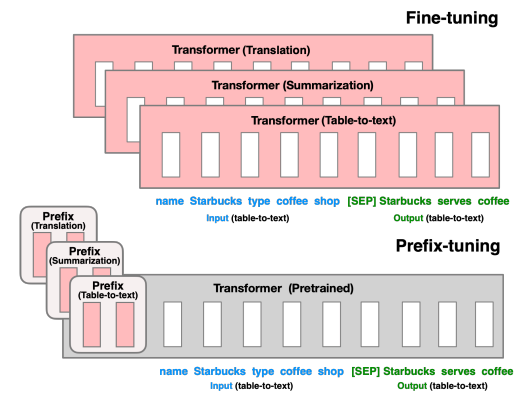
\includegraphics[width=0.6\textwidth]{prefix-tuning}
	\caption{Illustration of the prefix-tuning method, which freezes the Transformer parameters and only optimizes the prefix (the red prefix blocks). Consequently, it only needs to store the prefix for each task, making prefix-tuning modular and space-efficient. Note that each vertical block denote transformer activations at one time step. Source: \textcite{li2021prefixtuning}.}
	\label{fig:prefix-tuning}
\end{figure}
A novel approach to optimize prefix vectors involves using a re-parameterization technique, as described in the work by \textcite{li2021prefixtuning}.
This method employs a multilayer perceptron (MLP) function to map a smaller matrix to the parameter matrix of the prefixes, rather than directly optimizing the prefixes themselves.
This technique has proven effective for stabilizing the training process.
Once optimization is complete, the mapping function is discarded, leaving only the refined prefix vectors, which are tailored to enhance performance on specific tasks.
This approach leverages the inherent capabilities of the Transformer while only modifying a minimal set of parameters, making it modular and space-efficient.
\textcite{li2021prefixtuning} provides detailed empirical evaluations demonstrating that prefix-tuning achieves comparable performance to full fine-tuning while only learning about 0.1\% of the parameters.
Evaluations are performed on tasks like table-to-text generation and summarization using models such as GPT-2 and BART\@.
Results indicate that prefix-tuning not only reduces parameter count significantly but also maintains competitive performance with traditional fine-tuning in full data settings and often outperforms it in low-data scenarios.
The approach is particularly effective in handling tasks with unseen topics during training, showcasing better generalization capabilities~\cite{lewis2020bart}.


\subsubsection{Prompt tuning}
\label{subsubsec:prompt-tuning}

Prompt tuning primarily involves incorporating trainable vectors, called prompt tokens, at the input layer of a model.
These tokens, based on discrete prompting techniques, augment the input text to assist models in performing specific tasks.
In prompt tuning, these task-specific embeddings are combined with the original text embeddings and processed by language models.
Specifically, the method known as P-tuning employs a flexible approach to integrate context, prompt, and target tokens.
\begin{figure}[h!]
	\centering
	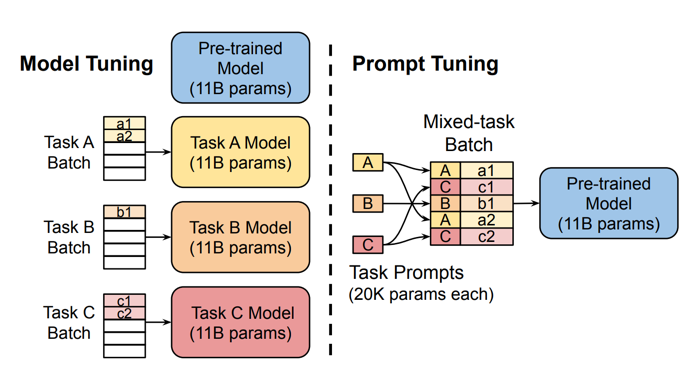
\includegraphics[width=0.8\textwidth]{prompt-tuning}
	\caption{Illustration of the prompt tuning method, which only requires storing a small task-specific prompt for each task, and enables mixed-task inference using the original pretrained model. With model tuning, each copy of tuned models requires copy billions of parameters, while tuned prompt would only requires thousands parameters per task---a reduction of over five orders of magnitude. Source: \textcite{lester2021power}.}
	\label{fig:prompt-tuning}
\end{figure}
This method is adaptable for tasks involving both understanding and generation of natural language and utilizes a bidirectional LSTM to learn representations of soft prompt tokens.
During the training phase, only these prompt embeddings are updated based on task-specific requirements.
The effectiveness of prompt tuning methods depends significantly on the computational power of the underlying language models, as they generally involve a limited number of trainable parameters at the input layer.

\textcite{liu2022ptuning} introduces P-Tuning v2, a method that extends prompt tuning by applying continuous prompts across all layers of a language model, improving upon the conventional method where prompts are only used at the input layer.
They address the limitations of traditional prompt tuning, which underperforms especially on complex sequence labeling tasks when model size is below 10 billion parameters~\cite{lester2021power}.
P-Tuning v2 modifies the conventional prompt tuning by:
\begin{itemize}
	\item Utilizing continuous prompts at every layer of the model to increase tunable parameter count without significantly increasing overall parameter load.
	\item Improving adaptability across both simple and complex tasks by modifying the interaction of prompts with model architecture~\cite{li2021prefixtuning, qin2021learning}.
\end{itemize}
P-Tuning v2 has been evaluated across a variety of model scales (from 330M to 10B parameters) and tasks including both classification and sequence labeling.
The experiments demonstrate that P-Tuning v2 provides comparable results to full model fine-tuning while requiring only 0.1\%-3\% of the parameters to be tuned.
\textcite{liu2022ptuning} concludes that P-Tuning v2 significantly narrows the performance gap between prompt tuning and full fine-tuning, offering a robust, scalable, and efficient alternative for adapting large pre-trained models to diverse NLU tasks.

\subsubsection{LoRA}
\label{subsubsec:lora}

The technique called LoRA (Low-Rank Adaptation) is used for efficient fine-tuning of neural networks, particularly in the adaptation of dense layers to downstream tasks with a reduced number of trainable parameters.
LoRA strategically freezes the original parameter matrix $W \in \R^{m \times n}$ and applies updates using a low-rank decomposition approach, which involves two smaller matrices $A \in \R^{m \times k}$ and $B \in \R^{n \times k}$ where $k$ is much smaller than $m$ or $n$.
This method significantly reduces the memory and storage requirements by limiting the number of trainable parameters to those in $A$ and $B$, rather than the entire matrix $W$.

The key advantage of LoRA is its ability to maintain a single large model while adapting it to various tasks using different sets of low-rank matrices for each task, enhancing storage efficiency and reducing computational costs.
Advanced methods for determining the optimal rank have been proposed such as importance score-based allocation~\cite{zhang2023adalora} -- i.e., AdaLoRA -- and search-free optimal rank selection~\cite{valipour2023dylora} -- DyLoRA\@.
These methods help to determine the optimal rank for the low-rank decomposition, ensuring that the model is adapted efficiently to the specific task requirements.

In AdaLoRA\footnote{Adaptive Low-Rank Adaptation} the idea is that adding more trainable parameters to the critical weight matrices can lead to better model performance.
In contrast, adding more parameters to those less important weight matrices yields very marginal gains or even hurt model performance.
Given the parameter budget, i.e., the number of total trainable parameters, AdaLoRA always prefer to allocate more parameters to those important modules.
Distributing the budget evenly to all weight matrices/layers, like LoRA and other methods (e.g., adapter and prefix
tuning), often gives suboptimal performance~\cite{zhang2023adalora}.
AdaLoRA operates by parameterizing the incremental updates in the form of singular value decomposition (SVD), allowing for selective pruning of updates based on their assessed importance.
This selective pruning targets the singular values of unimportant updates, effectively reducing their parameter budget while avoiding the computational intensity of performing exact SVD calculations.
SVD-based adaptation is represented as:

\begin{equation}
	W = W^{0} + \delta = W^{0} + P \Lambda Q
	\label{eq:svd-adaptation}
\end{equation}

\noindent where $W^{0}$ is the original parameter matrix, $\delta$ is the update, $P$ and $Q$ are the left and right singular vectors, and $\Lambda$ is the singular value matrix.
\textcite{zhang2023adalora} substantiates the effectiveness of AdaLoRA through extensive experiments across various NLP tasks, including question answering and natural language generation.
These experiments demonstrate notable improvements in performance, particularly in low-budget settings, when compared to baseline methods such as full fine-tuning and other parameter-efficient techniques like LoRA and adapter tuning.
Key benchmarks from the paper highlight AdaLoRA's superior performance on standard datasets like GLUE and SQuAD, where it consistently outperforms other approaches while utilizing fewer parameters.

DyLoRA\footnote{Dynamic Search-Free Low Rank Adaptation} is a search-free method for determining the optimal rank for low-rank decomposition in neural networks.
The method is based on the observation that the optimal rank for low-rank decomposition varies across different layers and tasks.
The main advantages of DyLoRA over conventional LoRA include its ability to adapt to different rank sizes dynamically during inference, eliminating the need for exhaustive search and re-training across different rank sizes.
This is achieved by training the low-rank modules (LoRA blocks) across a spectrum of ranks during the training phase, which allows the model to adjust to the best performing rank size at runtime without additional computational cost.
This method is inspired by the nested dropout technique but tailored to the needs of dynamic rank adaptation.
The implementation involves sampling a rank size during each training step and adjusting the adapter modules accordingly, which allows the model to learn to perform under various constraints of rank size efficiently.
Main improvements of DyLoRA over LoRA include:

\begin{enumerate}
	\item Dynamic LoRA Blocks: DyLoRA modifies the standard LoRA blocks to be dynamic, allowing them to adjust their rank size during inference. This adaptation leads to more flexible models that can perform well across a broader range of tasks without the need for specific tuning for each task.

	\item Search-Free Adaptation: By avoiding the exhaustive search for the optimal rank size, DyLoRA reduces the training and adaptation time significantly. The models can be trained once and used dynamically across different settings, making it highly efficient.

	\item Performance: Experimental results show that DyLoRA matches or exceeds the performance of traditional LoRA with a static rank across various NLP tasks. This is demonstrated in tasks such as sentiment analysis, question answering, and natural language generation, indicating the robustness and versatility of DyLoRA.

\end{enumerate}

\subsubsection{Memory-efficient model adaptation}
\label{subsubsec:memory-efficient}

In addition to parameter-efficient model adaptation, memory-efficient techniques have been proposed to reduce the memory footprint of LLMs.
These methods aim to reduce the memory requirements of LLMs during inference, making them more suitable for deployment in resource-constrained environments.
In this section, we discuss some of the most popular method for memory-efficient model adaptation, i.e.\ model quantization.

\subsubsection{Quantization}
\label{subsubsec:quantization}

Quantization techniques reduce memory and computational costs by representing weights and activations with lower-precision data types like 8-bit integers (int8).
This enables loading larger models you normally wouldn’t be able to fit into memory, and speeding up inference.
This process can lead to substantial reductions in both the storage requirements and the computational complexity of deploying LLMs, which is crucial for their application in resource-constrained environments.

Quantization can be done in two ways: post-training quantization and quantization-aware training.
Post-training quantization is done after the model has been trained, while quantization-aware training is done during training.
Post-training quantization is easier to implement, but quantization-aware training can lead to better results.

Main quantization techniques include: uniform quantization, non-uniform quantization, and mixed-precision quantization.
Uniform quantization maps the floating-point values to a fixed set of integer values, while non-uniform quantization uses a non-linear mapping to better represent the distribution of the data.
Mixed-precision quantization uses a combination of different precision data types to represent the weights and activations.

Uniform quantization discretizes the values within a certain range into equal-sized intervals.
Mathematically, it can be described as:

\begin{equation}
	\textbf{LinearQuant}(x, bitwidth) = \text{Clip}(\text{round}(\frac{x}{bitwidth}) \times bitwidth, minV, maxV)
	\label{eq:uniform-quantization}
\end{equation}

\noindent where minV and maxV are the minimum and maximum scale range respectively~\cite{hubara2017quantized}.

Non-uniform quantization, such as logarithmic quantization, allocates more fine-grained intervals to values that are more frequent or more sensitive to quantization errors.
This method can be represented as:

\begin{equation}
	\textbf{LogQuant}(x, bitwidth)(x) = \text{Clip}(\text{AP2}(x), minV, maxV)
	\label{eq:non-uniform-quantization}
\end{equation}

\noindent where AP2 is the approximate-power-of-2 function that maps the input to the nearest power of two as defined in \textcite{hubara2017quantized}.
This approach is particularly effective for distributions with a high dynamic range~\cite{miyashita2016convolutional}.

Mixed-precision quantization leverages the strengths of both uniform and non-uniform quantization by using different precision data types for different parts of the model.
For example, weights can be quantized to 8-bit integers while activations are quantized to 16-bit integers.

\begin{table}[htbp]
	\centering
	\begin{tabular}{ccc}
		\toprule
		Bit-width           & Storage Reduction & Accuracy Loss \\
		\midrule
		32 (Full Precision) & 0\%               & 0\%           \\
		16                  & 50\%              & 1\%           \\
		8                   & 75\%              & 2\%           \\
		4                   & 87.5\%            & 5\%           \\
		\bottomrule
	\end{tabular}
	\caption{Performance comparison of quantized LLM}
	\label{tab:quant_perf}
\end{table}

As per Table~\ref{tab:quant_perf}, lower bit-widths generally result in more significant storage savings, but they can also lead to higher accuracy losses~\cite{jacob2017quantization}.
